\cotefile{136}
\scanpage{282}
\margin{\unsure{1}}
\margin{282}
\begin{center}- 35 -\end{center}\hfill IX

On a un isomorphisme canonique (compatible aux opérations de $\pi$) :
\[
(*)\qquad H^1(A_{\overline K},\mathbb Z_\ell)\simeq\operatorname{Hom}(T_\ell(A(\overline K)),\mathbb Z_\ell)\quad,
\]
qui montre que l'assertion 3.7 équivaut à la même assertion pour les opérations de $I$ sur le premier membre de (*). Or cette assertion a été prouvée dans III\quad (en utilisant la résolution des singularités des schémas excellents de dimension 2).

\uline{Corollaire} 3.8. \uline{Les conditions équivalentes} (i) \uline{à} (iv) \uline{de} 3.5 \uline{équivalent aussi à la condition suivante} :

(vi) \uline{L'action de} $I$ \uline{sur} $U=T_\ell(A(\overline K))$ \uline{est unipotente}.

En effet, pour prouver que (v) implique (vi), on note que si un groupe $I$ opérant de façon unipotente sur un vectoriel $E$ de dimension finie sur un corps de caractéristique nulle (en l'occurrence $\mathbb Q_\ell$) admet un sous-groupe d'indice fini $I'$ opérant avec l'échelon $m$ (en l'occurrence $m=2$), alors $I$ lui-même opère avec l'échelon $m$. En effet, $I'$ étant d'indice fini dans $I$, le groupe algébrique $G'\subset\underline{\mathrm{Gl}}(E)$ qu'il définit est d'indice fini dans celui, $G$, défini par $I$, or $G$ étant unipotent est connexe (caractéristique nulle !), donc $G=G'$, donc $I$ et $I'$ ont même ``échelon d'unipotence''.

On obtient également une réciproque à 3.3 :

\uline{Corollaire} 3.9. \uline{Les notations sont celles de} 3.2. \uline{Les conditions} (i) \uline{et} (ii) \uline{de} 3.2 \uline{équivalent aussi à la condition suivante} :

(iii) \uline{Pour toute extension étale} $K'$ \uline{de} $K$, \uline{désignant par} $S'$ \uline{le normalisé de} $S$ \uline{dans} $K'$, \uline{par} $A'$ \uline{le modèle de Néron de} $A_{K'}=A\otimes_S K'=A_K\otimes_K K'$, \uline{le morphisme canonique}

\margin{353}
\margin{353}

\scanpage{283}
\diagram{\begin{tikzcd}
\cdots P \arrow[r] & C\otimes C' \arrow[r,shift left=.5ex] \arrow[r,shift right=.5ex] & C\otimes C'\otimes s
\end{tikzcd}}

\diagram{\begin{tikzcd}
V(P) & V(C\otimes\deleted{\unsure{s}}C') \arrow[l] \arrow[dl] & V(C)\times V(C')\times V(s) \arrow[l,shift left=.5ex] \arrow[l,shift right=.5ex] \\
V(C'') & &
\end{tikzcd}}

\[
P=\operatorname{Ker}\bigl(C\otimes C'\rightrightarrows C\unsure{\otimes_s|\otimes}C'\bigr)\deleted{\otimes s}\unsure{)}
\]
\[
P\deleted{\unsure{\otimes s}}\longrightarrow P\otimes s
=\operatorname{Ker}\bigl(\underbrace{C\otimes C'}\otimes s
\unsure{=|\rightrightarrows}\underbrace{C\otimes s\otimes C'}\otimes s\bigr)
\]
\diagram{\begin{tikzcd}P\arrow[r]&C\otimes C'\end{tikzcd}}
\diagram{\begin{tikzcd}P\otimes s\arrow[r]&C\otimes C'\otimes s\end{tikzcd}}

\diagram{\begin{tikzcd}
P\arrow[r,phantom,"{\overset{i}{\subset}}"]\arrow[d,"?"']&C\otimes C'\arrow[d,shift right=.6ex,"\alpha"']\arrow[d,shift left=.6ex,"\beta"]\\
P\otimes s\arrow[r,phantom,"{\overset{i\otimes\mathrm{id}_s}{\subset}}"]&C\otimes C'\otimes s
\end{tikzcd}}
\[
\alpha i=\beta i\overset{?}{=} (i\otimes\mathrm{id}_s)\circ\left(\underset{?}{\Delta_P}\right)
\]
\[
x\in C\otimes C'\qquad\alpha(x)=\beta(x)
\]
\[
\unsure{a}\in s
\]
\[
\alpha(x)=\beta(x)\quad\unsure{\longrightarrow}\quad\text{dans}\quad
\deleted{\unsure{\alpha}}\operatorname{Im}(\unsure{u}\otimes s\longrightarrow C\otimes C'\otimes s)
\]
\[
x\otimes s
\]

\diagram{\begin{tikzcd}[column sep=small]
&&C''\arrow[dl]\arrow[d]\arrow[dr]&\\
\cdots P_3\arrow[r,phantom,"\subset"]\arrow[d]&P_2\arrow[r,phantom,"\subset"]\arrow[d]&P_1\arrow[r,phantom,"\subset"]\arrow[dr]&C\otimes C'\arrow[d,shift right=.5ex,"\alpha"']\arrow[d,shift left=.5ex,"\beta"]\\
P_2\otimes s\arrow[r,phantom,"\subset"]&\unsure{P'_1|P_1}\otimes s\arrow[rr,phantom,"\subset"]&&C\otimes C'\otimes s
\end{tikzcd}}
\[
P
\]
\[
\deleted{\unsure{A}\otimes}\qquad
s^{\unsure{h|k}}\otimes_{\unsure{h|k}}s^{\unsure{h|k}}=s.
\qquad \unsure{\ne}
\]
\[
u\otimes1-1\otimes u
\]
\[
P_\infty=\bigcap P_i\qquad C''\subset C\otimes_k C'
\]
\diagram{\begin{tikzcd}P_\infty\deleted{\unsure{\otimes s}}\arrow[r]&C\otimes C'\otimes\unsure{e|s}\end{tikzcd}}
\[
\deleted{\underline M\otimes_k N}\qquad
u_C\otimes\mathrm{id}_{C'}=\mathrm{id}_C\otimes u_{C'}
\]
\[
x\otimes1-1\otimes x
\]
\[
x\otimes y-1\otimes xy
\]
\diagram{\begin{tikzcd}
P_\infty\arrow[dr]&\\
&\displaystyle\bigcap_i P_i\otimes s=P_\infty\otimes s
\end{tikzcd}}
\[
V(C)\boxtimes_{V(s)}V(C')
\]

\uline{\unsure{copr. dans les mod.}}

\diagram{\begin{tikzcd}C\arrow[r]&C\boxtimes_s C\end{tikzcd}}
\diagram{\begin{tikzcd}V(C)\times V(C'')\arrow[r,dash,"\unsure{-|\to}"]&V(C'')\end{tikzcd}}
\[
\unsure{V(s)\text{-équiv.}}
\]
\[
\deleted{M\otimes M'\otimes s\otimes s}
\]
\[
M\otimes s\qquad M'\otimes s
\]
\diagram{\begin{tikzcd}
\unsure{\Longleftrightarrow}\quad C''\arrow[r]&C\boxtimes C'\quad\text{\unsure{hom.} de \unsure{Co.algèbres}}
\end{tikzcd}}
\margin{283}

\scanpage{284}
\begin{center}- 32 -\end{center}\hfill IX

\uline{Proposition} 3.5. (\uline{critère galoisien de réduction semi-stable}). \uline{On suppose} $S$ \uline{un trait}. \uline{Les conditions suivantes sur le schéma abélien} $A_K$ \uline{sont équivalentes}\quad (\uline{les notations étant celles de} (2.5.3), \uline{appliquées à la situation déduite de} $(A_K,S)$ \uline{par passage au hensélisé de} $S$) :

(i) $A_K$ \uline{a réduction semi-stable sur} $S$ (3.4).

(ii) \uline{On a}, \uline{avec les notations} (2.5.3), (2.5.4) :
\[
V\subset V^\perp\quad.
\]
(iii) \uline{On a pour la partie torique} $W$ \uline{du module de Tate} :
\[
W=V^\perp\quad.
\]
(iv) \uline{L'action du groupe d'inertie} $I$ \uline{sur} $U=T_\ell(A(\overline K))$ \uline{est unipotente d'échelon} 2 (\uline{i.e.}\ \uline{il existe un sous-module} $U'$ \uline{de} $U$ \uline{stable par} $I$ \uline{tel que} $I$ \uline{opère trivialement sur} $U'$ \uline{et sur} $U/U'$).

On peut supposer $S$ hensélien (3.4.0). Avec les notations de 2.1.9, (i) signifie que l'on a
\[
\lambda=0\quad,
\]
ce qui en vertu de (2.5.5) équivaut à $V=V\cap V^\perp$ i.e. à (ii). Comme $W=V\cap V^\perp$ par le théorème d'orthogonalité 2.4, on a (ii) $\Longleftrightarrow$ (iii). D'ailleurs (iv) signifie aussi que $I$ opère trivialement sur $U^I\unsure{=|\ne}V$, ce qui par dualité signifie qu'il opère trivialement sur $V^\perp$ i.e. que $V^\perp\subset U^I=V$, ce qui est (ii). Cela achève la démonstration.
\margin{\unsure{q}}

\uline{Remarques} 3.5.1. Les conditions (ii) et (iv) ne dépendent visiblement que de l'action de $I$ sur le $\mathbb Q_\ell$-vectoriel $U\otimes_{\mathbb Z_\ell}\mathbb Q_\ell$, et auraient pu être formulées en termes de cette action. Signalons aussi que ces conditions sont manifestement stables par tout changement de base par un morphisme
\margin{\unsure{?}\quad\unsure{\supset}}

\margin{350}
\margin{350}
\margin{284}

\scanpage{285}
\diagram{\begin{tikzcd}
s\arrow[r,"\Delta_s"]&s\otimes s&\\
C\arrow[u,"\unsure{\varphi}"']\arrow[r,"\Delta_C"]&C\otimes C\arrow[u]\arrow[r,"{\mathrm{id}_C\otimes\unsure{\varphi}}"]&C\otimes s
\end{tikzcd}}

$V(s)$ \unsure{anneau} opère sur $V(C)$

$V(C)$ structure d'\unsure{algèbre} sur $V(s)$ ?

\diagram{\begin{tikzcd}
V(C)\unsure{\times|\otimes}_{\deleted{\unsure{V(s)}}}V(C')\arrow[r,"{\text{bil. p.r. à }V(s)}"']&V(C'')
\end{tikzcd}}

1°) bil. p.r. à \deleted{$V(s)$} $\unsure{\mathcal O|0}$ \unsure{donc correspond} :
\diagram{\begin{tikzcd}C''\arrow[r]&C\otimes_{\unsure{k|h}}C'\end{tikzcd}}

\diagram{\begin{tikzcd}
V(C)\times V(s)\times V(C')\arrow[r,"{\mathrm{id}_{V(C)}\times\omega_{V(C')}}"]\arrow[d,"{\deleted{\unsure{\omega_{V(C)}\times\mathrm{id}_{V(s)}}}}"']&V(C)\times V(C')\arrow[d]\\
V(C'')\times V(s)\arrow[r]&V(C'')
\end{tikzcd}}

\diagram{\begin{tikzcd}
&\phantom{C''}\\
&C''\arrow[u,"{\deleted{\unsure{\sim}}}"]\\
V(C)\times\operatorname{Spec}(A)\arrow[r]&V(C'')
\end{tikzcd}}
\diagram{\begin{tikzcd}V(C)\arrow[r]&V(C'')\end{tikzcd}}
\[
\deleted{V(C)\times V(s)\times\operatorname{Spec}(A)}
\]

\diagram{\begin{tikzcd}
C&C''\arrow[l]\arrow[d]\\
C\otimes s\arrow[u,phantom,"{\unsure{\downarrow|\uparrow}}"]&C''\otimes s\arrow[l]
\end{tikzcd}}
\diagram{\begin{tikzcd}C\otimes A&C''\arrow[l]\end{tikzcd}}

\diagram{\begin{tikzcd}
V(C)\times V(C')\arrow[r,no head]&V(C'')\\
\operatorname{Sym}(C)\otimes\operatorname{Sym}(C')&C''\arrow[l]
\end{tikzcd}}

\diagram{\begin{tikzcd}
C''\arrow[r,no head]\arrow[d]&C\otimes A\arrow[d,phantom,"{\unsure{\downarrow|\uparrow}}"]\\
C''\otimes s\arrow[r]&C\otimes s\otimes A
\end{tikzcd}}

\diagram{\begin{tikzcd}[column sep=small]
&\deleted{C\otimes\operatorname{Sym}(C')\unsure{\longrightarrow}}\arrow[dl]\\
\Delta_C\otimes\mathrm{id}_{\unsure{C''|C'}}\simeq\mathrm{id}_C\otimes\Delta_{C'}&\\
\simeq(\alpha\otimes\mathrm{id}_s)\circ\Delta_{C''}&
\end{tikzcd}}

\diagram{\begin{tikzcd}
C''\arrow[r,"\alpha"]\arrow[d,"\Delta_{C''}"']&C\otimes C'\arrow[d,"{\Delta_C\otimes\mathrm{id}_{C'}}"]\\
C''\otimes s\arrow[r,"{\alpha\otimes\mathrm{id}_s}"]&C\otimes s\otimes C'
\end{tikzcd}}
\figure{\begin{tikzpicture}\draw[->] (0,1) .. controls (1,.8) and (1,.25) .. (.45,0);\end{tikzpicture}}
\figure{\begin{tikzpicture}\draw (0,2) .. controls (.5,2) and (.5,1.5) .. (.5,1) -- (.5,.3) .. controls (.5,.1) and (.6,0) .. (.7,0);\end{tikzpicture}}
\margin{285}

\scanpage{286}
\begin{center}- 103 -\end{center}\hfill IX

canonique de $(\check M'\otimes_{\mathbb Z}\check M)\otimes_{\mathbb Z}\mathbb Z_\ell$, d'ailleurs invariant par $\pi_o=\pi/I=\operatorname{Gal}(\overline k/k)$, puisque par définition il est invariant par transport de structure :
\[
(9.2.9)\qquad u\in(\check M'\otimes_{\mathbb Z}\check M)\otimes_{\mathbb Z}\mathbb Z_\ell)^I
\simeq\operatorname{Hom}_{\mathbb Z}(\underline M\otimes\underline M';\mathbb Z_\ell)
\simeq\operatorname{Hom}_{\mathbb Z_\ell}(\underline M_\ell\otimes\underline M'_\ell,\mathbb Z_\ell)\quad.
\]
C'est (à la notation $u$ au lieu de $u_\ell$ près) l'élément (9.1.2) que nous voulions définir.

Pour définir (9.1.2) dans le cas général, nous aurons besoin de quelques préliminaires, que nous allons développer dans les deux sections suivantes .

9.3. \uline{Extensions panachées}.

Soient $\underline C$ une catégorie abélienne, et
\[
(9.3.1)\qquad P,\ R,\ Q
\]
trois objets de $\underline C$. On s'intéresse à la classification des objets $X$ de $\underline C$, munie d'une filtration en trois crans
\[
(*)\qquad X^o=X\supset X^1\supset X^2\supset X^3=0\quad,
\]
avec des isomorphismes donnés
\[
X^o/X^1\overset{\sim}{\longrightarrow}P\quad,\quad
X^1/X^2\overset{\sim}{\longrightarrow}R,\quad
X^2/X^3=X^2\overset{\sim}{\longrightarrow}Q\quad.
\]
Posant
\[
E=X^o/X^2\quad,\quad F=X^1/X^3=X^1\quad,
\]
on voit que $X$ donne naissance à deux extensions ordinaires

(9.3.2)
\diagram{\begin{tikzcd}[column sep=small]0\arrow[r]&P\arrow[r]&F\arrow[r]&R\arrow[r]&0\end{tikzcd}}
\quad,\quad
\diagram{\begin{tikzcd}[column sep=small]0\arrow[r]&R\arrow[r]&E\arrow[r]&Q\arrow[r]&0\end{tikzcd}}
\quad,

de $R$ par $P$ et de $Q$ par $R$ respectivement. Notre point de vue sera ici

\margin{421}
\margin{421}
\margin{286}

\scanpage{287}
(1) $S$ anneau \inserted{$\mathbb Z$-}gradué \inserted{comm} \uline{à degrés $\geq0$}, $S=\sum_{n\geq0}S_n^{\unsure{b|h}}$

\deleted{$\unsure{S_0=k}$}

(2) $k=S_0^{\unsure{b|h}}$

(3) $\operatorname{Modgr.d}(S)=\mathcal M$

(4) $\underline t$ foncteur translation
\[
(4.1)\quad\left\{\begin{array}{l}
\underline t:\mathcal M\unsure{\mathrel{-}|\longrightarrow}\mathcal M\\
\underline t(M)_i=M_{i+1}
\end{array}\right.
\]
\margin{c'est un \uline{automorphisme} de $\mathcal M$}
\[
(4.2)\qquad M[i]=\underline t^{\,i}(M).
\]
\deleted{\unsure{Il en va}}
Pour tout entier $N$, on considère les deux sous-catégories \inserted{str.} pleines \inserted{$\mathcal M_N,\mathcal M^N$} de $\mathcal M$ \unsure{définies} par
\[
(5)\quad\left\{\begin{array}{l}
\operatorname{Ob}\mathcal M_N=\{P\in\operatorname{Ob}\mathcal M\mid P_i=0\quad\forall i<N\}\\
\operatorname{Ob}\mathcal M^N=\{P\in\operatorname{Ob}\mathcal M\mid P_i=0\quad\forall i\unsure{>|\geq}N\}
\end{array}\right.
\]
\uline{NB} Les $\mathcal M_N$ ($\mathcal M^N$) décroissent (croissent) pour $N$ croissant. On a
\[
(6)\quad\left\{\begin{array}{l}
t^i(\mathcal M_N)=\mathcal M_{N-i}\\
t^i(\mathcal M^N]=\mathcal M^{N-i}_{\deleted{\unsure{N-i}}}
\end{array}\right.
\]
\deleted{\unsure{donc}}
En particulier \deleted{\unsure{et}}
\[
(6.1)\quad\left\{\begin{array}{l}
\deleted{\unsure{t}}\mathcal M_N=t^{-N}\mathcal M_0\quad,\\
\mathcal M^N=t^{-N}\mathcal M^0
\end{array}\right.
\]
\inserted{Dans} La catégorie $\mathcal M$, munie déjà de l'\unsure{autom.} $t$, la donnée des familles $(\mathcal M_N)$ et $(\mathcal M^N)$ avec leurs inclusions \unsure{définies}
\[
(7)\qquad\mathcal M_N\supset\mathcal M_{N'}\quad\text{et}\quad\mathcal M^N\subset\mathcal M^{N'}\quad\text{si}\quad N\leq N'
\]
équivaut à celle \deleted{\unsure{des}} du couple
\[
(\unsure{8|7})\qquad\mathcal M_0,\mathcal M^0\quad\text{avec}\quad t\mathcal M_0\unsure{\subset|\supset}\mathcal M_0,\quad
 t\mathcal M^0_{\deleted{\unsure{0}}}\supset\mathcal M^0_{\deleted{\unsure{0}}}
\]
\unsure{On va voir} d'ailleurs comment $\mathcal M_N,\mathcal M^{N-1}$ (\deleted{\unsure{ou encore $\mathcal M_N$, $\mathcal M^N$}}) se déterminent mutuellement -- donc $\mathcal M_0\unsure{\simeq|\text{ou}}\mathcal M^0$ permet de \unsure{retrouver} tous \deleted{\unsure{les}} $\mathcal M_N,\mathcal M^N$.

\margin{288}

\scanpage{288}
\begin{center}- 102 -\end{center}\hfill IX

Or par le théorème d'orthogonalité appliqué a la fois pour $A_K$ et $A'_K$ on a
\[
V^\perp=W\quad,\quad(U/V)^\vee\simeq W'(-1)\quad,
\]
où $W'$ est la partie torique de $U'=T_\ell(A'(\overline K))$, et où le $(-1)$ désigne le twist de Tate. D'autre part, l'homomorphisme (9.2.4) se factorise par $I(\ell)\simeq\mathbb Z_\ell(1)$, de sorte que l'homomorphisme (9.2.4) peut s'interpréter comme un homomorphisme canonique
\[
(9.2.5)\qquad u:\mathbb Z_\ell(1)\longrightarrow W'\otimes W(-1)\quad,
\]
ou encore comme un élément
\[
(9.2.6)\qquad u\in W'\otimes W(-2)\quad.
\]
Se rappelant de la définition de $W$ et de $W'$, comme les groupes de points à valeurs dans $\overline K$ des deux faisceaux $\ell$-adiques constants tordus $T_\ell(A^o)^t$ et $T_\ell(A'^o)^t$, dont les fibres spéciales sont respectivement $T_\ell(T_o)$ et $T_\ell(T'_o)$, on trouve les isomorphismes canoniques
\[
(9.2.7)\quad\left\{\begin{array}{l}
W\simeq T_\ell(T_o)(\overline k))\simeq\check M\otimes\mathbb Z_\ell(1)\\[1.5ex]
W'\simeq T_\ell(T_o(\overline k))\simeq M'\otimes\mathbb Z_\ell(1)\quad,
\end{array}\right.
\]
$M$ et $M'$ désignant les groupes des caractères relativement à $\overline k$ de $T_o$ et de $T'_o$ respectivement :
\[
(9.2.8)\qquad T_o=D(M)\quad,\quad T'_o=D(M')\quad.
\]
Par suite, l'élément $u$ de (9.2.6), qui exprime l'opération du groupe d'inertie $I$ sur le module de Tate $U$ de $A_K$, s'interprète comme un élément

\margin{420}
\margin{420}
\margin{289}

\scanpage{289}
On considère les foncteurs d'inclusion
\[
(9)\qquad i_N:\mathcal M_N\hookrightarrow\mathcal M\qquad
 i^N_{\deleted{\unsure{N}}}:\mathcal M^N\unsure{-|\longrightarrow}\mathcal M
\]
plus \uline{généralement}, pour $N\leq N'$
\[
(9.1)\qquad i_{N,N'}:\mathcal M_{N'}\hookrightarrow\mathcal M_N\qquad
 i^{N',N}:\mathcal M^N\subset\mathcal M^{N'}
\]
\deleted{On va étudier les}

\unsure{donc} :
\[
(9.2)\qquad i_Ni_{N,N'}=i_{N'\deleted{\unsure{,N}}}\quad,\qquad
 i^{N'}i^{N',N}=i^N
\]
\deleted{\unsure{plus g.}} et si $N\leq N'\leq N''$,\quad \unsure{d'où} \deleted{$\unsure{i_N}$}
\[
(9.3)\quad\left\{\begin{array}{ll}
\mathcal M_{N''}\subset\mathcal M_{N'}\subset\mathcal M_N\ \deleted{\text{et}}&\mathcal M^N\subset\mathcal M^{N'}\subset\mathcal M^{N''}\\[1ex]
i_{N,N''}=i_{N,N'}i_{N',N''}&i^{N'',N}=i^{N'',N'}i^{N',N}
\end{array}\right.
\]
On va étudier la suite de foncteurs adjoints associés à $i_N,i_{N,N'}$ d'une part, $i^N,i^{N,N'}$ d'autre part.

\uline{Proposition} 1 $i_N$\inserted{$:\mathcal M_N\hookrightarrow\mathcal M$} s'insère dans une suite de 4 foncteurs adjoints
\[
(10)\qquad q_N\quad i_N\quad\tau_N\quad\varphi_N
\]
(chaque foncteur \deleted{\unsure{est}} parmi $i_N,\tau_N,\varphi_N$ est adjoint à droite de celui écrit à sa gauche)

définis ainsi :
\[
a)\quad\tau_N:\mathcal M\longrightarrow\mathcal M_N\qquad
\text{(foncteur tronquage à droite)}
\]
\[
\tau_N(P)\inserted{i_N\tau_N(P)}\subset\deleted{\unsure{P}}P\qquad\text{(sous objet de }P\text{)}.
\]
\margin{hom d'adjonction}
\[
(10.1)\qquad(\tau_N(P))_i=\left\{\begin{array}{ll}P_i&\text{si }i\geq N\\0&\text{si }i<N\end{array}\right.
\]
\margin{290}

\scanpage{290}
\begin{center}- 101 -\end{center}\hfill IX

envisagé dans (2.5.3), et plus précisément, nous verrons que sa connaissance équivaut essentiellement à celle de l'action du groupe de monodromie $I$ sur $U$.

9.2. \uline{Cas} $\ell\ne p$ . Plaçons nous donc d'abord dans le cas, plus simple, où $\ell\ne p$, en reprenant alors les notations introduites dans (2.5.3). Notons qu'à torsion près, la relation $V=U^I$ signifie aussi que $V^\perp$ est le module engendré par les éléments $gx-x$ ($u\in U$, $g\in I$), et qu'on a en tous cas
\[
(9.2.1)\qquad gx-x\in V^\perp\quad\text{pour }x\in U,\ g\in I\quad.
\]
On a donc, pour $g\in I$ :
\[
(9.2.2)\qquad gx=x+u(g).x\quad,
\]
où $g\longmapsto u(g)$ est un homomorphisme de $U$ dans $V^\perp$ qui s'annule sur $V=U^I$, ou ce qui revient au même
\[
(9.2.3)\qquad u\in\operatorname{Hom}(U/V,\ V^\perp)\simeq(U/V)^\vee\otimes V^\perp\quad.
\]
Dans le cas envisagé de la réduction semi-stable, i.e. quand on a $V^\perp\subset V$, la formule (9.2.2) exprime que l'opération $g$ dans $U$ est une \uline{transvection} parallèle à $V^\perp=W$, et la composition de ces transvections n'est autre que l'addition des homomorphismes $u$ correspondants (9.2.3). Donc l'opération du groupe d'inertie $I$ sur $U$ s'explicite entièrement alors par un homomorphisme de groupes
\[
(9.2.4)\qquad I\longrightarrow(U/V)^\vee\otimes V^\perp\quad.
\]
\margin{$\longleftarrow$}
\margin{\unsure{419}}
\margin{419}
\margin{291}

\scanpage{291}
\[
b)\quad\varphi_N:\mathcal M_N\longrightarrow\mathcal M
\]
\[
(10.2)\quad\left\{\begin{array}{l}
(\varphi_N(Q))_i=\operatorname{Hom}^i_{\mathcal M}(\tau_{N-i}(S),Q\inserted{i_NQ})
\bigl(\longrightarrow\operatorname{Hom}^i_{\mathcal M}(S,Q)=Q_i\bigr)\\
\hspace{4em}=\operatorname{Hom}^{\unsure{b|0}}_{\mathcal M}(\tau_{N-i}(S)[-i],Q)
\end{array}\right.
\]
Avec \deleted{\unsure{leur}} structure de module provenant (pour $k\in\mathbb Z$, $u\in S_k^{\unsure{b|h}}$) des opérateurs ``multiplication par $u$'' :
\diagram{\begin{tikzcd}\tau_{N-i}(S)&\tau_{N-i-k}(S)\arrow[l,"{\text{deg }k}"]\end{tikzcd}}
en transposant; on a un hom (\unsure{dans} \deleted{\unsure{mod}} $\mathcal M$ décrit dans (10.2)
\[
(10.2.1)\qquad\varphi_N(Q)\longrightarrow i_N(Q)
\]
d'où en appliquant $\tau_N$
\[
(10.2.2)\qquad\tau_N\varphi_NQ\underset{\text{adj.}}{\overset{\sim}{\longrightarrow}}Q
\]
qui est un isom (c'est un hom d'\unsure{adjoint})

L'autre hom d'adjonction
\diagram{\begin{tikzcd}
\deleted{\varphi_N\tau_NP\longleftarrow}&P\arrow[r]&\varphi_N\tau_NP
\end{tikzcd}}
est \unsure{déduit|défini} des \deleted{\unsure{l'inclusion}} \inserted{hom}
\[
\deleted{\tau_NP\longrightarrow P}\qquad\operatorname{Hom}^i_{\mathcal M}(\tau_{N-\deleted{\unsure{i}}}S,P)
\]
(10.2.3)
\diagram{\begin{tikzcd}[column sep=small]
P_i\arrow[r]\arrow[dr,"\unsure{\sim|2}"']&(\varphi_N\tau_NP)_i\simeq\operatorname{Hom}^i(\tau_{N-i}S,\tau_NP)\\
&\operatorname{Hom}^i(S,P)\arrow[u]
\end{tikzcd}}
\margin{tout hom de degré $i$ \deleted{de $S$ dans $P$} $\tau_{N-i}S$ dans $P$ est à valeurs dans $\tau_{N\deleted{\unsure{-i}}}P\subset P$}

c) (NB On n'utilisera pas $q_N$, on le met par acquit de conscience) :
\[
q_N(P)=P/\text{sous-module engendré par les }P_i\text{ pour }i<N
\]
\margin{292}

\scanpage{292}
et que ces suites et la suite constante de valeur 1 forment une base de \unsure{l'espace} vectoriel $E_r$ de toutes les suites complexes de période $r$. Montrer que la série
\[
u(s)_n c_n
\]
est alternée à valeurs absolues décroissantes tendant vers zéro, donc convergente. En déduire une autre démonstration de b).

d) Soit $z$ un nombre complexe, et posons $u_n=z^n$ pour $n\quad1$. Montrer que la suite des sommes partielles $S_n$ de (1) reste bornée si et seulement si on a
\[
(5)\qquad z\quad1\ ,\quad z\ne1
\]
(auquel cas la suite des $S_n$ est majorée par $2\,\frac{z}{1-z}$).
\deleted{\unsure{Montrer que si la série $c_n$ est divergente, alors}}
\inserted{En déduire que} la condition (5) implique que la série \inserted{$c_nz^n$}\deleted{$\unsure{s_n|u_n}$} est convergente. Montrer qu'elle est même absolument convergente pour $z\quad1$, tandis que pour un $z$ tel que $z=1$, $z\ne1$, on a convergence absolue si et seulement si la \deleted{suite} série $c_n$ est convergente. Enfin,
\deleted{Application à la \unsure{convergence} \illegible{3} \unsure{Montrer que}}
\inserted{$A$ désignant une partie}\deleted{\unsure{pour toute partie $A$}} de l'ensemble \inserted{$E$} des nombres complexes satisfaisant (5), pour que la convergence de la série $c_nz^n$ soit uniforme pour $z\quad A$, il suffit qu'il existe un nombre $a\quad0$ tel que $z\quad A$ implique $1-z\quad a$. Montrer que cette condition est aussi nécessaire si la série $c_n$ est divergente (tandis que si $c_n$ est convergente, la convergence est uniforme pour l'ensemble des nombres complexes $z$ tels que $z\quad1$). \deleted{\unsure{E}}

e) Montrer que la fonction $f(z)$ sur l'ensemble $E$ des nombres complexes $z$ satisfaisant (5), représentée par la série
\[
(6)\qquad f(z)=c_nz^n
\]
est continue. Elle admet une limite finie pour $z=1$ si et seulement si la \deleted{suite} série $c_n$ est convergente, auquel cas la fonction $f(z)$ définie par la formule (6) est définie et continue \deleted{pour} sur tout le disque unité $z\quad1$.

f) Appliquer les résultats de d) et e) à la série trigonométrique
\[
c_ne^{ix}\quad,
\]
et aux séries
\[
c_n\cos nx\ ,\quad c_n\sin nx\quad;
\]
en particulier, ces séries sont convergentes pour tout $x$ réel n'appartenant pas à l'ensemble \deleted{$\unsure{\mathbb R}$} $2\quad\underline{\mathrm Z}$ (i.e. $x$ pas de la forme $2\ n$, avec $n$ entier), et représentent des fonctions continues de $x$ pour $x\quad\underline{\mathrm R}-2\quad\underline{\mathrm Z}$.

g) Montrer que la suite $(z^n)_{n\quad1}$ ($z$ étant un nombre complexe) est périodique de période $r$ si et seulement si $z$ est une racine $r$.ème de l'unité. \deleted{\unsure{En déduire}} Déduire de ceci et et b) que lorsque $z$ est une racine de l'unité la série \deleted{$\unsure{u_n}$} $c\ z$ est convergente, sauf dans le cas où $z=1$ et $c_n$ \unsure{est}

\margin{293}

\scanpage{293}
\uline{\unsure{Cor}})

Les foncteurs $i_N,\tau_N$ commutent à \unsure{ttes|toutes} les sortes de limites inductives et projectives, $q_N$ commute aux $\underset{\longrightarrow}{\lim}$, $\varphi_N$ aux $\underset{\longleftarrow}{\lim}$.

Les foncteurs $i_N,\varphi_N$ sont pl. fid., les foncteurs $q_N,\tau_N$ sont des foncteurs localisation. \deleted{\unsure{Comme}} Pour $\tau_N$ (puisque il est exact, et commute aux $\underset{\longrightarrow}{\lim}$ et $\underset{\longleftarrow}{\lim}$) c'est la localisation mod une sous-cat. abélienne épaisse, stable par $\underset{\longrightarrow}{\lim}$ et $\underset{\longleftarrow}{\lim}$; en fait, c'est précisément la sous-cat $\mathcal M^{N-1}$ (qui est ainsi décrite \deleted{\unsure{ici}} en termes de $\mathcal M_N$).

\margin{\figure{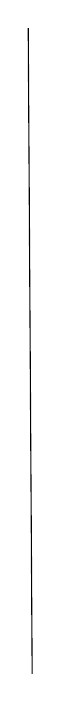
\begin{tikzpicture}\draw (0,0)--(-.05,8.2);\end{tikzpicture}}}
\margin{294}

\scanpage{294}
\begin{center}Problème MP 2\end{center}

Un des objets du présent exercice est d'étudier la convergence de certaines séries de la forme
\[ u_n/n\ , \]
où $(u_n)$ est une suite bornée de nombres complexes, et d'en calculer la somme dans certains cas, notamment dans le cas où la suite $(u_n)$ admet une ``période'' $r$ (de sorte qu'on a $u_{n+r}=u_n$ pour tout $r$).

I

Soit $(c_n)_{n\quad1}$ une suite décroissante de nombres positifs tendant vers
\deleted{\unsure{$0$, et soit $u_n$}}
$0$, et soit $(u_n)_{n\quad1}$ une suite de nombres complexes. \inserted{a)} On suppose qu'il existe un nombre $M\quad0$ tel que pour tout entier $n\quad0$, on a
\[ S_n=\mathop{\quad}_{1\quad i\quad n}u_i\quad M\ . \]
\deleted{a)} Prouver que la série
\[ u_nc_n \]
est convergente, et que pour tout entier $n\quad1$, le reste
\[ R_n=\mathop{\quad}_{i\quad n+1}u_ic_i \]
satisfait
\[ R_n\quad Mc_{n+1}\ . \]
(Utiliser le critère de Cauchy, en prouvant que pour $m\quad n$, on a
\[ \mathop{\quad}_{n\quad i\quad m}u_ic_i\quad Mc_{n+1}\ ; \]
pour ceci, remplacer dans le premier membre $c_i$ par $S_i-S_{i-1}$.)

b) On suppose que la suite $(u_n)$ est périodique de période $r$ ($r\quad1$), et on s'intéresse à la convergence de la série $u_nc_n$. Montrer que si la série $c_n$ est convergente, il en est de même de $u_nc_n$ quelle que soit la suite (périodique) $(u_n)$. Montrer que si la série $c_n$ est divergente, alors $u_nc_n$ est convergente si et seulement si on a
\[ \mathop{\quad}_{1\quad i\quad r}u_i=0\unsure{/}\ . \]
(Montrer que toute suite $(u_n)$ périodique de période $r$ se met de façon unique sous forme d'une somme de deux suites périodiques de période $r$
\[ u_n=u'_n+u''_n\ , \]
où $(u'_n)$ est une suite constante et où $(u''_n)$ satisfait à la condition
\[ \mathop{\quad}_{1\quad i\quad r}u''_i=0\ . \]
Appliquer alors le résultat de a) à cette dernière suite.)

c) On considère l'espace \inserted{vectoriel complexe $E_r$} des suites périodiques \inserted{$u=$} $(u_n)$ de période $r$ satisfaisant la condition (3). Soit $n_0\quad1$, et soit, pour tout entier \unsure{$s$} tel que $1\quad\unsure{s}\quad r-1$, $u(\unsure{s})=(u(\unsure{s})_n)_{n\quad1}$ l'unique suite $\quad E_r$ telle qu'on ait
\deleted{$\unsure{u(i)_{n\quad r}}$}
pour $0\quad i\quad r-1$,
\[
u(\unsure{s})_{n_0+i}=
\begin{array}{ll}
1&\text{si }\deleted{\unsure{i=s,\ 0\ \text{pour}\ i\ne s}}\ i=0\\
-1&\text{si }i=s\\
0&\text{si }i\ne0,s
\end{array}\ .
\]
Prouver que les $u(s)$ ($1\quad s\quad r-1$) forment une base de l'espace vectoriel

\margin{295}

\scanpage{295}
$C$ cat. abélienne

$S$ anneau $\mathbb Z$-gradué comm. à degrés $\geq0$

$\mathcal M$ \inserted{$=\mathcal M(C,S)$} catégorie des $C$-$S$-modules gr. \uline{\unsure{diffs.}}

$\mathcal M_N$, $\mathcal M^N$ définis comme plus haut.

\diagram{\begin{tikzcd}\mathcal M_N\arrow[r,"i_N"]&\mathcal M\end{tikzcd}}

admet \deleted{foncteur} adjoint à droite

\diagram{\begin{tikzcd}\mathcal M\arrow[r,"\tau_N"]&\mathcal M_N\end{tikzcd}}
\[ i_N\tau_N(P)\subset P \]

\deleted{qui admet}

Construire adjoint à droite $\varphi_N$ de $\tau_N$ :
\[
\operatorname{Hom}_{\mathcal M_N}(\tau_NP,\underset{\in\mathcal M_N}{Q})\simeq
\operatorname{Hom}_{\mathcal M}(P,\varphi_NQ)\ ?
\]
\margin{\unsure{1}}

Il faut \unsure{donc} prouver que pour $Q$ fixé, le premier mb, comme foncteur en $P$, est repr. Or il est clair que $\tau_N$ commute aux $\varinjlim$ qui sont \unsure{représent.bles} dans $\mathcal M$ donc le foncteur du premier mb transforme ces $\varinjlim$ en $\varprojlim$. Cela implique donc ce qu'on veut lorsque $C$ \uline{ou} $C^o$ est une ``cat. de Groth''\ldots

Comment \inserted{alors} décrire les $(\varphi_NQ)_i\in\operatorname{Ob}C$

On a pour tout $M\in\operatorname{Ob}\mathcal M$
\[ M_i\simeq\underline{\operatorname{Hom}}^*(S,M)_i \]
donc
\[
\begin{aligned}
(\varphi_NQ)_i&=\underline{\operatorname{Hom}}^*(S,\varphi_NQ)_i
\simeq\underline{\operatorname{Hom}}^*(S[-i],\varphi_NQ)_0\\
&\overset{\unsure{\text{quid pro}}}{=}\underline{\operatorname{Hom}}^*(\tau_N(S[-i]),Q)_0\\
&=(\underline{\operatorname{Hom}}^*((\tau_{N-i}(S))[-i],Q)\deleted{\unsure{\tau_N}})_0
\end{aligned}
\]
\margin{296}

\scanpage{296}
\begin{center}- 100 -\end{center}\hfill IX

9. \uline{Définition de l'accouplement de monodromie} $\underline M_\ell\otimes\underline M'_\ell\longrightarrow\mathbb Z_{\ell S}$.

9.1. Dans le présent numéro on suppose $S$ hensélien, et que $A_K$ ait réduction semi-stable sur $S$, ou ce qui revient au même, que $A'_K$ ait réduction semi-stable sur $S$ (3.5.1). On dispose alors sur $S$ de deux $\mathbb Z$-Modules constants tordus $\underline M$ et $M'$ (5.5.2), qui sur un revêtement fini étale convenable de $S$ (donc sur $S$ lui-même si $S$ est strictement local i.e. si $k$ est séparablement clos) se déploient en des groupes constants de valeur $M$ resp. $M'$ isomorphes (non canoniquement) à $\mathbb Z^r$, $r$ étant la dimension commune des tores maximaux de $A_o$ et de $A'_o$. Nous allons considérer, pour tout nombre premier $\ell$, les faisceaux $\ell$-adiques correspondants
\[
\tag{9.1.1}\underline M_\ell=\underline M\otimes_{\mathbb Z}\mathbb Z_\ell\ ,\quad
\underline M'_\ell=\underline M'\otimes_{\mathbb Z}\mathbb Z_\ell\ ,
\]
dont la signification géométrique est explicitée par les formules (5.5.7) et (5.5.8). Dans le présent numéro, nous allons définir un accouplement canonique (dit ``\uline{accouplement de monodromie}'')
\[
\tag{9.1.2}u_\ell:\underline M_\ell\otimes\underline M'_\ell\longrightarrow\mathbb Z_\ell\ ,
\]
qui sera défini en termes des pro-$\ell$-groupes de Barsotti-Tate $T_\ell(A^o)$ et $T_\ell(A'^o)$, et même de la fibre générique $T_\ell(A_K)$ du premier de ces groupes (sous réserve, lorsque $\ell=p$, de disposer du théorème de Tate [33, th.4], i.e. pour l'instant qu'on soit alors dans le cas d'inégales caractéristiques). Lorsque $\ell\ne p$, il revient au même de dire que l'accouplement (9.1.2) est décrit en termes du $\pi$-module galoisien
\[
\tag{9.1.3}U=T_\ell(A_K)(\overline K)=T_\ell(A_{\overline K})
\]
\margin{$\unsure{\ni}\qquad\unsure{u}$}
\margin{\figure{\begin{tikzpicture}\draw (0,0)--(.23,-.25);\draw (0,-.7)--(.3,-.72);\end{tikzpicture}}}
\margin{\unsure{418}}
\margin{418}
\margin{297}

\scanpage{297}
\[
\begin{aligned}
&\deleted{=(\underline{\operatorname{Hom}}^*((\tau_NS))[-i],Q))_0}\\
&\deleted{=\underline{\operatorname{Hom}}^*(\tau_{N-i}S}\\
&\simeq(\underline{\operatorname{Hom}}^*(\tau_{N-i}(S),Q))_i\\
&\simeq\underline{\operatorname{Hom}}^i(\tau_{N-i}(S),Q)
\end{aligned}
\]

Enfin si dans $C$ les $\unsure{\underline{\lim}|\varinjlim}$ existent, alors $i_N$ admet un adjoint à gauche $q_N$.

En dualisant (appliquant ce qui précède à $C^o$, en utilisant l'isom

\diagram{\begin{tikzcd}
\mathcal M(C,S)^o\arrow[r,phantom,"\simeq"]\arrow[d]&\mathcal M(C^o,S)\arrow[d]\\
\mathcal M^N_{\deleted{\unsure{N}}}(C,S)^o\arrow[r,phantom,"\simeq"]&\mathcal M_{\leq N}(C^o,S)
\end{tikzcd}}

on voit que (si $\unsure{C,\ C^o}$ est une cat. de Groth. p ex) le foncteur
\[ i^N:\mathcal M^N\longrightarrow\mathcal M \]
\deleted{admet} \inserted{s'insère dans} une suite \deleted{\unsure{d'adj.}} \inserted{de 4} foncteurs adjoints
\[ \varphi^N\ \tau^N\ i^N\ q^N \]
qui se décrivent de façon duale.

\margin{298}

\scanpage{298}
\margin{299}
\begin{center}- 34 -\end{center}\hfill IX

On observera que $S'$ est noethérien régulier connexe de dimension 1, ce qui donne un sens à la conclusion énoncée. Pour prouver 3.6, choisissons une clôture séparable $\overline K$ de $K$, et écrivons l'extension $\overline K$ comme limite inductive de ses sous-extensions galoisiennes finies $K_i$. Soit $S_i$ le normalisé de $S$ dans $K_i$, et soit $U$ le plus grand ouvert de $S$ sur lequel $A_K$ ait bonne réduction. Comme $S$ est noethérien connexe de dimension 1, et $U\ne\varnothing$, on voit que $T=S-U$ est un ensemble fini de point fermés de $S$, et que pour tout $t\in T$, $\underline O_{S,t}$ est un anneau de valuation discrète. Il suffit de trouver, pour tout $t\in T$, un indice $i=i(t)$ tel que $A_{K_i}$ ait réduction semi-stable en les points de $S_i$ au-dessus de $t$ ; en effet, il suffira de prendre alors pour $K'$ le composé des extensions $K_{i(t)}$ pour $t\in T$. Cela nous ramène donc au cas où $S$ est un trait. D'autre part, comme de groupe $\operatorname{Gal}(K'/K)$ permute entre eux les points de $S_i$ au-dessus du point fermé $s$ de $S$, il suffit de trouver $K'$ de telle façon que $A_{K'}$ ait réduction semi-stable en \uline{un} point du normalisé $S'$ ; d'ailleurs il est inutile ici que $K'$ soit galoisien sur $K$, il suffit de trouver $K'$ extension finie étale de $K$ satisfaisant la condition précédente, car la clôture galoisienne de cette extension satisfera à la même condition. Utilisant le critère 3.5 (iv) on voit donc que 3.6 revient à l'assertion suivante :

\uline{Corollaire} 3.7. \uline{On suppose à nouveau} $S$ \uline{un trait}. \uline{Alors il existe un sous-groupe ouvert} $\pi'$ \uline{de} $\pi$ \uline{tel que l'action} $I'=I\cap\pi'$ \uline{sur} $U=T_\ell(A(\overline K))$ \uline{soit unipotente d'échelon} 2, \uline{ou encore} : \uline{il existe un sous-groupe ouvert} $I'$ \uline{de} $I$ \uline{dont l'action sur} $U$ \uline{soit unipotente d'échelon} 2.

\margin{352}
\margin{352}

\scanpage{299}
\deleted{$\unsure{\delta\in\mathbb Z},\ \beta\geq0,$}
$\alpha,\beta\geq0$, $d\geq\beta-\alpha$

\diagram{\begin{tikzcd}[column sep=large,row sep=large]
\operatorname{Hom}^d(\tau_{\deleted{\unsure{\beta}}\alpha}M_{S_h},\tau_\beta N_{S_h})
\arrow[r,"\sim","{\substack{\alpha'\geq\alpha\\\beta'\geq\beta\\(\deleted{\unsure{\text{exact}}}\\\beta'-\alpha'\geq d)}}"']
&\operatorname{Hom}^d(\tau_{\deleted{\unsure{\beta'}}\alpha'}M_{S_h},\tau_{\beta'}N_{S_h})
\arrow[d,"\sim","{\gamma\geq\unsure{\beta}-d\ (\text{si }d\leq0)}"']\\
&\operatorname{Hom}^d(\tau_\gamma M,N)
\arrow[d,phantom,"\simeq"{rotate=90}]
&{\substack{(\text{ou bien }\operatorname{Hom}^d(M,\tau_{\unsure{\delta}}N)\\\text{si }0\leq\unsure{\delta}\leq d,}}\\
&\operatorname{Hom}^d(M_{\unsure{S_h}},\varphi_\beta\tau_\beta N_{S_h})\ (\text{si }d\leq0)
\arrow[d,phantom,"\simeq"{rotate=90}]\\
&\operatorname{Hom}^d(S_h,\varphi_0((\unsure{\operatorname{Hom}_h}(M,N)_{S_h})))
\arrow[d,phantom,"\simeq"{rotate=90}]\\
&(\varphi_0(\operatorname{Hom}_h(M,N)_{S_h}))_d
\end{tikzcd}}

$M_{\deleted{\unsure{g}}}$ $h$-module
\[ M_{S_h}=M\otimes_h h\{T\} \]
\[
(\varphi_0M_{S_h})_{-d}\simeq
\underset{\substack{\begin{tikzpicture}[baseline=-.5ex]\node[rotate=90] {$\in$};\end{tikzpicture}\\u}}{\operatorname{Hom}^{-d}(\tau_dS_h,M_{S_h})}
\]
\[ u(T^{(i)})=\xi_i T^{(i-d)}\qquad(i\geq d)\qquad\xi_i\in M \]
\[
u(\underbrace{T^{(i)}T^{\unsure{(\ell)|\ell}}}_{c_{i\ell}T^{(i+\ell)}})
=c_{i\ell}\xi_{i+\ell}T^{(\unsure{i-\ell-d|i+\ell-d})}
\]
\margin{\figure{\begin{tikzpicture}\draw[->] (0,.4)--(-.2,0);\end{tikzpicture}}}
\[
u(T^{(i)})T^{\unsure{(\ell)|\ell}}=\xi_i T^{(i-d)}T^{\unsure{(\ell)|\ell}}
=c_{i-d,\ell}\xi_i T^{(\unsure{i-\ell-d|i+\ell-d})}
\]
\[
i\geq d,\ \ell\geq0\quad\Longrightarrow\quad
\boxed{c_{i,\ell}\xi_{i+\ell}=c_{i-d,\ell}\xi_i}
\]
\[ c_{d,\ell}\xi_{d+\ell}=\xi_d \]
\margin{300}

\scanpage{300}
\margin{301}
\begin{center}- 160 -\end{center}\hfill IX

d'entiers $[1,r]$), $D_\lambda$ étant l'image par $\underline f:\underline X\longrightarrow\underline S$ de la composante $D'_\lambda$ passant par le point singulier $x_\lambda$ de $X_o$ du lieu de non lissité $D'=\bigcup_{\lambda\in L}D'_\lambda$ du morphisme $\underline f$. Par construction même, $f:X\longrightarrow S$ est isomorphe à l'image inverse de $\underline f:\underline X\longrightarrow\underline S$ par un $W$-morphisme convenable $g:S\longrightarrow\underline S$ :

(12.8.2)
\diagram{\begin{tikzcd}
\underline X\arrow[d,"\underline f"']&X\arrow[l]\arrow[d,"f"]\\
\underline S&S\arrow[l,"g"]
\end{tikzcd}}.

Posons
\[\tag{12.8.3} P=\underline{\operatorname{Pic}}^o_{\underline X/\underline S}\ ;\]
comme la fibre spéciale de $\underline f$ est géométriquement réduite de dimension 1, il s'ensuit que $\underline F$ est cohomologiquement plat en dimension 0 (EGA III 7.8.1) et que $P$\unsure{-est} formellement lisse sur $S$ (ce dernier fait résultant de ce que $H^2(X_o,\underline O_{X_o})=0$, $X_o$ étant de dimension 1). Pour simplifier, nous allons admettre que $P$ \uline{est représentable par un schéma en groupes sur} $S$ (qui sera nécessairement un schéma en groupes lisse à fibres connexes) ; c'est là un cas particulier d'un résultat inédit de MUMFORD cité dans [22](considérablement généralisé par RAYNAUD dans la note citée, dans le cas où la base est un trait). Comme aucune démonstration des résultats de MUMFORD ni de RAYNAUD n'a été publiée, le lecteur préférera peut-être utiliser les résultats généraux de M. ARTIN [1], qui donnent la représentabilité de $P$ (sous la seule hypothèse de partir d'un $\underline f$ propre, plat et cohomologiquement plat en dimension 0) par un ``espace algébrique''

\margin{\unsure{1}}
\margin{\unsure{t}}
\margin{\figure{\begin{tikzpicture}\draw (0,0)--(.05,.4);\draw (.22,.47)--(.32,.41);\draw (.7,.9)--(.71,1.12);\end{tikzpicture}}}
\margin{478}

\scanpage{301}
\begin{flushright}
\unsure{Notations|Notions} $\tfrac12$ simpliciales

Constructions universelles
\end{flushright}
\margin{\figure{\begin{tikzpicture}\draw (0,0) rectangle (.28,.28);\end{tikzpicture}}}
\margin{302}

\scanpage{302}
\mspage{1}
\margin{1975\quad\unsure{à}\quad1976}
\[
\boldsymbol\Delta=\text{cat. des simplexes }\Delta^n\quad(n\geq0)
\]
\margin{$\Delta^n=[0,n]\subset\mathbb N$\quad avec rel. d'ordre \unsure{total|totale}}
\[
\widehat{\boldsymbol\Delta}=\mathrm{Ss}=\underline{\operatorname{Hom}}(\boldsymbol\Delta^o,\mathrm{Ens})=\mathrm{Ens}_*
\]
Plus généralement, si $A$ est une catégorie, on pose
\[
\begin{aligned}
A_*&=\underline{\operatorname{Hom}}(\boldsymbol\Delta^o,\mathrm{Ens})\\
A^*&=\underline{\operatorname{Hom}}(\boldsymbol\Delta,\mathrm{Ens})
\end{aligned}
\]
donc
\[ (A^o)^*=(A_*)^o\qquad A^*\simeq((A^o)_*)^o \]
où l'exposant $o$ désigne le \inserted{\unsure{passage à la}} cat. opposée.

Les objets de $A_*$ (resp. $A^*$) sont considérés comme des structures algébriques de type simple (sur une infinité d'objets de base) dans $A$, les ``objets $\tfrac12$ simpliciaux'' resp. ``$\tfrac12$ cosimpliciaux''. On écrira $\mathrm{Ens}_*$ quand on a en vue cet aspect, et $\widehat{\boldsymbol\Delta}$ \inserted{ou $\mathrm{Ss}$} quand on a plutôt le \unsure{p\textsuperscript{t}} de vue ``objet d'un topos'' ou ``faisceau sur un topos'' $\unsure{\flat}$. Tous les développements qui suivront ont pour objet d'étudier ces objets (l'équivalent combinatoire des espaces topologiques) et leurs ``types d'homotopie'', \unsure{i.e.} des invariants qu'on peut leur associer, qui en dépendent de façon covariante ou contravariante. Nous avons ici en vue une étude systématique, dans l'esprit de l'algèbre universelle, de ces invariants, (qui sont donc des foncteurs sur $\widehat{\boldsymbol\Delta}\simeq\mathrm{Ens}_*$) \deleted{et des} \inserted{de leurs structures et des} opérations qui peuvent être définies sur elles, permettant d'en déduire certains complexes \unsure{à} partir \unsure{d'autres} plus simples

\margin{$\unsure{\flat}$ La notation $\widehat{\boldsymbol\Delta}$ peut être utilisée de préf. quand on veut garder à l'esprit la nature \uline{algébrique} très particulière de ces \unsure{types}, la notation $\mathrm{Ss}$ quand on veut l'oublier au profit de la \uline{signification} topologique.}
\margin{303}

\scanpage{303}
\mspage{2}
Un objet de $A_*$ sera généralement noté par un symbole de la forme $K_*$, où $K_*$ désigne la famille des
\[ K_*(\Delta^n)=K_{[n]} \]
avec les opérations $\tfrac12$ simpliciales entre elles.
\margin{par abus de notation $K_*=(K_{[n]})_{n\geq0}$ ou mieux $\Delta^n\longmapsto K_{[n]}$}
On fera attention qu'on écrit $K_{[n]}$ et non $K_n$, pour des raisons qui vont apparaître (impérieuses lorsque $A$ est additive\ldots).
De même un objet de $A^*$ sera noté
\[ K^*=(n\longmapsto K^{[n]})\overset{\text{abus.}}{=}(K^{[n]})_n \]

Nous aurons à travailler avec la situation, où on a deux catégories $A$ et $B$, et une équivalence (notée \deleted{$\unsure{\vee^*}$} $M\mapsto M^\vee$)
\[ \vee:A^o\overset\simeq\longrightarrow B\qquad\text{d'où }B^o\simeq A \]
[le plus souvent $A=B$ et $(M^\vee)^\vee\underset{\substack{\text{isom}\\\text{fonct.}}}{\simeq}M$, avec compatibilités habituelles d'une autodualité\ldots]
on notera alors \inserted{souvent} par la \unsure{m\textsuperscript{e}} lettre un objet de $A_*$ (ou $A^*$) et l'objet de $A^*$ (resp. $A_*$) qui lui correspond par application de $\vee$, mais en indiquant la variance par la position du \uline{signe} $*$
\[
\begin{array}{ll}
K^*=(K_*)^\vee&K^{[n]}={K_{[n]}}^\vee\\
K_*=(K^*)^\vee&K_{[n]}={K^{[n]}}^\vee
\end{array}
\]

On s'intéressera surtout au cas où ($h$ étant un anneau fixé) \deleted{$\unsure{A=\mathcal L}$}
\deleted{$\unsure{A:\ A}$}
\[
\begin{aligned}
A&=\deleted{\unsure{\mathrm{Ab}_h}}\ h\text{-modules à g. proj. d.t.f.}\\
B&=h\text{-modules à droite proj. de t.f.}
\end{aligned}
\]
(si $h$ est commutatif, on a $A=B$ et on a une autodualité dans $A$).

On a le foncteur canonique pl. fid
\diagram{\begin{tikzcd}(*)\quad\boldsymbol\Delta\arrow[r,hook]&\widehat{\boldsymbol\Delta}=\mathrm{Ss}\end{tikzcd}}
l'image par ce foncteur de $\Delta^n$ est noté ${\Delta^n}_*$ \inserted{ou mieux ${\Delta^{[n]}}_*$ (puisqu'il est covariant en $n$)}. On a donc
\[
{\Delta^n}_*\ (\text{ou }{\Delta^{[n]}}_*)=(m\longmapsto{\Delta^n}_{[m]}=\operatorname{Hom}_{\mathrm{Ens}}(\Delta^m,\Delta^n))
\]
et pour $\unsure{X}_*\in\operatorname{Ob}\widehat{\boldsymbol\Delta}$,
\[
\operatorname{Hom}({\Delta^n}_*,\unsure{X}_*)\simeq X_*(\Delta^n)\simeq X_{[n]}
\]
en particulier
\[
\operatorname{Hom}({\Delta^n}_*,{\Delta^m}_*)\simeq{\Delta^m}_*({\Delta^n}_*)\simeq\operatorname{Hom}_{\boldsymbol\Delta}(\Delta^n,\Delta^m)
\]
\margin{$\Vert\quad(\operatorname{Hom}_{\mathrm{ord}}(\Delta^n,\Delta^m))$}
Pour $n$ variable, ${\Delta^n}_*\in\widehat{\boldsymbol\Delta}$ dépend de façon \uline{covariante} de $n$, \deleted{\unsure{(i.e. on}} donc le foncteur $n\longmapsto{\Delta^n}_*$ (qui n'est autre que (*)) est un objet canonique de $\widehat{\boldsymbol\Delta}^*$, qu'on appellera \uline{objet cosimplicial universel} et noté $\Delta^*$ (ou mieux ${\Delta^*}_*${)}
\[
{\Delta^*}_*\in\widehat{\boldsymbol\Delta}^*=(\mathrm{Ens}_*)^*\qquad\text{donc }\forall n\geq0
\]
\[
{\Delta^{[n]}}_*\in\widehat{\boldsymbol\Delta}\qquad
{\Delta^{[n]}}_*={\Delta^n}_*=m\longmapsto
\underset{\substack{\Vert\\\operatorname{Hom}_{\boldsymbol\Delta}(\Delta^n,\Delta^m)}}{{\Delta^n}_{[m]}}
\]
\deleted{\unsure{Elle}}
[Une parenthèse de notations : Considérons les catégories de la forme $(A_*)^*$, un objet de \unsure{là-dedans} est donc noté $K^*=(K^{[n]})_n$, où les $K^{[n]}$ sont des $\in A_*$, donc s'écrivent ${K^{[n]}}_*$,
\[ {K^{[n]}}_*=({K^{[n]}}_{[m]})_{m\geq0} \]
Ainsi, on est amené à noter ${K^*}_* $ les objets de $(A_*)^*\simeq\underline{\operatorname{Hom}}(\boldsymbol\Delta\times\boldsymbol\Delta^o,A$
\deleted{\unsure{on}}

\margin{304}

\scanpage{304}
\mspage{3}
\[ {K^{[m]}}_{[n]}=K(\Delta^m,\Delta^n)\in A \]
De \unsure{m\textsuperscript{e}}, on note
\[
\begin{aligned}
{K_*}^*&\quad\text{les objets de }(A^*)_*\simeq\underline{\operatorname{Hom}}(\boldsymbol\Delta^o\times\boldsymbol\Delta,A)\\
K^{**}&\quad\text{les objets de }(A^*)^*\simeq\underline{\operatorname{Hom}}(\unsure{\boldsymbol\Delta^o|\boldsymbol\Delta}\times\boldsymbol\Delta,A)\\
K_{**}&\quad\text{les objets de }A_{**}=\underline{\operatorname{Hom}}(\boldsymbol\Delta^o\times\boldsymbol\Delta^o,A)
\end{aligned}
\]

On fera attention que si on compose avec l'un des foncteurs de symétrie
\deleted{$(m,n)\longmapsto(n,m)$}
\inserted{$(\Delta^m,\Delta^n)\longmapsto(\Delta^n,\Delta^m)$}
dans $\boldsymbol\Delta\times\boldsymbol\Delta$ ou dans $\boldsymbol\Delta^o\times\boldsymbol\Delta^o$, ou entre $\boldsymbol\Delta\times\boldsymbol\Delta^o$ et $\boldsymbol\Delta^o\times\boldsymbol\Delta$), on n'utilisera pas la même lettre pour désigner un \deleted{complexe} \inserted{objet} (tel que ${K^*}_*$ ou $K^{**}$ disons) ou son transformé (qui devrait alors s'écrire ${K_*}^*$, ou encore une fois $K^{**}$), car cela conflicterait avec la convention plus haut de la ``montée et descente des indices''
\[ {K_*}^*\simeq({K^*}_*)^\vee \]
dans le premier cas, et \deleted{\unsure{serait}} amènerait à écrire
\[ K^{[m][n]}=K^{[n][m]} \]
dans le deuxième ! On utilisera au besoin un symbole ``de symétrie'' tel que $\sigma$, pour dénoter le symétrique de $K$ ($={K^*}_*,K^{**}$) par
\[ {}^\sigma K\ (= {({}^\sigma K)_*}^*,({}^\sigma K)^{**}) \]
\deleted{\unsure{de}} \ldots D'ailleurs,
\deleted{Ces considérations et notations}
si on a un objet ${K^*}_*$ disons, \inserted{$\in\operatorname{Ob}(A^{\deleted{\unsure{*}}}_*)^*_{\deleted{\unsure{*}}}$} alors pour $\forall n\geq0$, on peut considérer
\[
\deleted{\unsure{u\longmapsto}}\quad
{K^*}_{[n]}\overset{\mathrm{def}}{=}(m\longmapsto {K^{[m]}}_{[n]})
\]
comme un objet de $A^*$ ; le foncteur $[n]\longmapsto {K^*}_{[n]}$ de ${A^*}_*$ n'est autre que ${}^\sigma K$.
On étend ces considérations et notations au cas de symboles $K$ à plus de deux indices, pour désigner des objets de catégories de

\margin{305}

\scanpage{305}
\mspage{4}
de la forme
\[
 {{A^*}_*}^{**}=\bigl(( (A^*)_* )^*\bigr)^*
 \deleted{\unsure{ce sont}}\quad\text{p.ex.}
\]
--- dont les objets sont notés par des lettres à étoiles
$ {{K^{**}}_{**}}^*\ldots\ \Big]$

Le rôle de ${\Delta^*}_{\unsure{*}}\in\operatorname{Ob}\widehat{\boldsymbol\Delta}^{*}$
\inserted{$=\operatorname{Ob}Ss^*$}
comme ``objet cosimplicial universel'' est explicité par la

\uline{Proposition 1}. Soit $A$ une catégorie où les $\underline{\lim}$ existent
(resp. $B$ une catégorie où les $\varprojlim$ existent). Alors
\[
 \text{a)}\quad A^*\xleftarrow{\approx}
 \underline{\operatorname{Hom}}_{\text{comm. à }\varinjlim}(Ss,A)
\]
par $F\longmapsto F(\Delta^*)$
\[
 \text{b)}\quad B_*\xleftarrow{\sim}
 \underline{\operatorname{Hom}}_{\text{comm. à }\varprojlim}(Ss^o,B)
\]
par $F\longmapsto F((\Delta^*)^o)$

(où $(\Delta^*)^o$ désigne l'objet simplicial de $\widehat{\boldsymbol\Delta}^{o}$
défini par l'objet cosimplicial $\Delta^*$ de $\widehat{\boldsymbol\Delta}$).

Bien sûr, b) n'est autre que a) appliqué à $A=B^o$, et a) signifie que
le foncteur ``restriction à $\boldsymbol\Delta$''
\[
 \underline{\operatorname{Hom}}(\widehat{\boldsymbol\Delta},A)
 \longrightarrow\underline{\operatorname{Hom}}(\boldsymbol\Delta,A)
\]
induit une équivalence sur la ss-cat
\deleted{\unsure{des}}\inserted{comm. à $\underline{\lim}$}
du premier mb. C'est vrai pour \uline{ttes}
(\deleted{petites}\inserted{\unsure{nos}}) catégories $C$ ---
pas seulement pour $\boldsymbol\Delta$, et bien connu.
Le foncteur en sens inverse associe, à
$K_*=\varphi:\boldsymbol\Delta\mathbin{\text{---}}A$, le foncteur
\[
 X_*\longmapsto
 \underset{\Delta^n_*\in\boldsymbol\Delta/X_*}{\underline{\lim}}
 \varphi(\Delta^n_*)=
 \underset{\Delta^n_*\in\boldsymbol\Delta/X_*}{\underline{\lim}}K_{[n]}
\]
Dans le cas b) où on \unsure{écrit}
\[
 \underline{\operatorname{Hom}}(\widehat{\boldsymbol\Delta}^{o},B)
 \longrightarrow\underline{\operatorname{Hom}}(\boldsymbol\Delta^{o},B)
\]
le foncteur en sens inverse associe à
$K^*=\psi:\boldsymbol\Delta^o\mathbin{\text{---}}B$
le foncteur contravariant
\[
 X^*\longmapsto
 \varprojlim_{\Delta^n_*\in(\boldsymbol\Delta/X_*)^o}\varphi(\Delta^n)
 =\varprojlim_{\Delta^n\in(\boldsymbol\Delta/X_*)^o}K^{[n]}
\]

\uline{Yoga}: nous nous intéresserons surtout
\deleted{aux} (en première étape) aux invariants covariants attachés à $X_*$,
à valeurs dans une cat. $A$, qui \deleted{pour $X_*$}\inserted{commutent}
aux $\underline{\lim}$ p.r. à $X_*$, --- ils sont donc déterminés
(si $A$ est ``\uline{\unsure{grosse|grande}}'' pour contenir les $\underline{\lim}$
(petites)) par des éléments de $A^*$ i.e. des objets \uline{cosimpliciaux} de $A$.
Pour les invariants contravariants en $X_*$, à val. dans un $B$, nous nous
attacherons en premier lieu à ceux qui \deleted{commutent} aux $\varprojlim$
en $X_*$; pour $B$ stable par $\varprojlim$, ils correspondent
\deleted{donc} aux objets de $\underline B_*$, i.e. les objets
$\tfrac12$ simpliciaux de $B$. Si $B=(Ens)$, cela correspond donc à des
ens. $\tfrac12$ simpliciaux, i.e. à des objets $K_*$ de
$\unsure{Ss|B}$ lui-même.
\margin{306}

\scanpage{306}
\mspage{5}\deleted{\unsure{5}}
Ce n'est autre que le foncteur représenté par $K_*$, et on le notera aussi
\[
 \deleted{\unsure{K_*(X_*)=}}
 \qquad X_*\longmapsto K_*(X_*)=\operatorname{Hom}(X_*,K_*)
\]
Si $B=(Ab)$, $K_*$ sera de même un objet de $Ss_{ab}$
\deleted{$\unsure{Ab_*}$}, et en effet le foncteur qu'il représente est
automatiquement muni de \deleted{\unsure{structure}}\inserted{\unsure{groupe Abélien}}
\unsure{additive|addition}. $\overline M$ remarque pour les structures
\uline{algébriques} (sur un ou plusieurs objets de base) qui
``puissent s'exprimer en termes de $\varprojlim$ exclusivement''
(gps, \deleted{\unsure{anneaux}}, anneaux, modules sur
\deleted{\unsure{des anneaux}}\deleted{\unsure{etc.}} etc.).

\uline{Rem}. Les \deleted{foncteurs} invariants ainsi obtenus,
à coups de foncteurs représent.bles --- plus génér., d'objets simpliciaux
ou cosimpliciaux de catégories $B$ ou $A$ --- sont de nature trop
``grosse'' et ``fruste'' pour être intéressants directement --- en
particulier, ce ne sont pas des invariants du type d'homotopie de $X_*$.
On devra en extraire des invariants plus subtils qui soient des invariants
du type d'homotopie de $X_*$, --- ceux-ci ne seront pas de nature si simple
--- i.e. ``repr.'' par des objets simpliciaux ou cosimpliciaux.
Notre propos sera de mettre sur les invariants ``gros'' qu'on vient de décrire,
un maximum de structures supplémentaires remarquables, et dans les catégories
de structures de ce type (complexes de chaînes ou de cochaînes, algèbres
cosimpliciales etc.) d'inverser les flèches qu'on obtient à partir d'équiv.
d'homotopie des $Ss$, et de passer à des ``catégories de fractions'' en
inversant ces flèches. L'invariant ainsi obtenu
\deleted{\unsure{deviendra}}\inserted{(plus ``grossier''}
bien sûr, mais plus subtil dans sa définition, et moins ``redondant'')
\unsure{exprimera|exprime} donc de façon plus ou moins complète le type
d'homotopie, ou en saisira de façon adéquate tels ou tels aspects.

Dans le cas où $A$ est une catégorie additive karoubienne (tout projecteur
dans un objet a un noyau, ou ce qui revient au même, tt proj. a un conoyau)
le th.\unsure{ème|éorème} de Dold-Puppe donne des équivalences canoniques
\diagram{\begin{tikzcd}[column sep=large]
 A_*\arrow[r,shift left=1ex,"{\mathrm{ND}_{\cdot}}","\approx"']&
 A_{\cdot}\arrow[l,shift left=1ex,"{\mathrm{DP}_*}","\approx"']
\end{tikzcd}},
\margin{$\mathrm{ND}=$ ``non-dégénéré''\\$\mathrm{DP}=$ ``Dold-Puppe''}
où $A_{\cdot}$ désigne la catégorie des \uline{complexes de chaînes}
dans $A$. On désigne par une même lettre \inserted{telle $K$} deux objets
qui se correspondent, mais en mettant en indice soit $*$ soit $\cdot$,
suivant qu'il
\margin{307}

\scanpage{307}
\mspage{6}
s'agit de désigner \unsure{l'aspect en} ``objet simplicial'' ou ``complexe de chaînes'':
\[
 K_{\cdot}=\mathrm{ND}_{\cdot}(K_*),\qquad K_*=\mathrm{DP}_*(K_{\cdot})
\]
\[
 K_*=(n\mathrel{\unsure{\vdash|\mapsto}}K_{[n]}),\qquad
 K_{\cdot}=(K_n,d_n)_{n\geq0}
\]
On est ainsi amené à noter par une notation $K_{\cdot}$ tt complexe de chaînes,
par $K_n$ ses composantes (ce qui exclut l'utilisation de la notation $K_n$
pour la $n$.ième composante \inserted{de} $K_*$, et nous oblige à adopter
une notation telle que $K_{[n]}$!).

De même, le \unsure{th.ème|théorème} de $\mathrm{DP}$ appliqué à $A^o$ nous donne des équivalences
\diagram{\begin{tikzcd}[column sep=large]
 A^*\arrow[r,shift left=1ex,"{\mathrm{ND}^{\cdot}}","\approx"']&
 A^{\cdot}\arrow[l,shift left=1ex,"{\mathrm{DP}^*}","\approx"']
\end{tikzcd}}
et des notations
\[
 K^{\cdot}=\mathrm{ND}^{\cdot}(K^*),\qquad K^*=\mathrm{DP}^*(K^{\cdot})
\]
\[
 K^{*}_{\deleted{\unsure{*}}}=(n\mathrel{\unsure{\vdash|\mapsto}}K^{[n]}),\qquad
 K^{\cdot}=(K^n,d^n)_{n\geq0}.
\]
Les foncteurs $\mathrm{ND}^{\cdot}$ et $\mathrm{DP}^*$ commutent aux foncteurs additifs.
En particulier, dans le cas d'une équivalence
\diagram{\begin{tikzcd}[column sep=large]
 A\arrow[r,leftrightarrow,"\approx","\vee"']&B^o
\end{tikzcd}}
déjà envisagé, étendant aux complexes de chaînes ou de cochaînes la convent.
de la montée ou de la descente des indices, on trouve que les foncteurs
$\mathrm{ND}$ et $\mathrm{DP}$ y commutent. Donc dans ce cas, la même lettre $K$ désigne
\margin{308}

\scanpage{308}
\mspage{7}
quatre avatars possibles
\[
 K^*\quad K_*\quad K^{\cdot}\quad K_{\cdot}
\]
liés par les relations ci-dessus
\[
 \left\{\begin{array}{ll}
 K^*=\mathrm{DP}^*(K^{\cdot})&K^{\cdot}=\mathrm{ND}^{\cdot}(K^*)\\
 K_*=\mathrm{DP}_*(K_{\cdot})&K_{\cdot}=\mathrm{ND}_{\cdot}(K_*)
 \end{array}\right.
\]
plus les relations
\[
 \left\{\begin{array}{ll}
 K^*=(K_*)^\vee,&K_*=(K^*)^\vee\\
 K^{\cdot}=(K_{\cdot})^\vee,&K_{\cdot}=(K^{\cdot})^\vee.
 \end{array}\right.
\]
\deleted{\unsure{(et leur signification}}

Ces \deleted{$\unsure{K^*=}$} notations et remarques (i.e. équivalences de
catégories) s'étendent aux objets \deleted{\unsure{simpliciaux}}
\inserted{dépendant de} plusieurs indices, p.ex \deleted{$\unsure{K^*}$}
une même lettre $K$, désignant \inserted{\unsure{initialemt|initialement}}
un objet ${K^*}_*$ de $(A_*)^*$ \inserted{disons}, désigne également,
\deleted{\unsure{un objet}} quatre avatars distincts
\[
 \left\{\begin{array}{ll}
 {K^*}_*\in(A_*)^*,&({K^{\cdot}}_*)\in(A^{\deleted{\unsure{*}}}_*)^{\cdot}\\
 {K^{\cdot}}_{\cdot}\in(A_{\cdot})^{\cdot},&({K^*}_{\cdot})\in(A_{\cdot})^*
 \end{array}\right.
\]
avec des notations
\[
 \begin{array}{ll}
 {K^{[n]}}_{[m]},&{K^n}_{[m]}\\
 {K^n}_m,&{K^{[n]}}_m
 \end{array}
\]
pour les composantes. De même, on aura, si on part p.ex. de
$K^{**}\in(A^*)^*$
\[
 \left\{\begin{array}{ll}
 K^{**}\in(A^*)^*,&K^{\unsure{\cdot}*}\in(A^{\cdot})^*\\
 K^{\cdot\cdot}\in(A^{\cdot})^{\cdot},&K^{*\cdot}\in(A^*)^{\cdot}
 \end{array}\right.
\]
\[
 \left\{\begin{array}{ll}
 K^{[n][m]},&K^{n[m]}\\
 K^{nm},&K^{[n]m}
 \end{array}\right.
\]
On notera qu'un objet de $(A_*)^{\cdot}$ est un complexe de cochaînes
\inserted{$n\longmapsto({K_*}^{n},d^n)$}
dans la catég. $A_*$ des objets $\tfrac12$ simpliciaux de $A$,
\margin{309}

\scanpage{309}
\mspage{8}
ou encore (moyennant l'équivalence de catégories canonique
\[
 \sigma:(A_*)^{\cdot}\simeq(A^{\cdot})_*\qquad)
\]
un objet $\tfrac12$ simplicial dans la catégorie $A^{\cdot}$ des complexes
de cochaînes, soit
\[
 n\longmapsto {K_{[n]}}^{\cdot}.
\]
On interprète de même les objets des autres catégories mixtes
\deleted{\unsure{$\tfrac12$ simplic. $A^{\cdot*}$}}
\[
 (\unsure{*|R})\quad
 \left\{\begin{array}{llll}
 A_{*\cdot},&A_{\cdot*},&{A^{*\deleted{\unsure{*}}}}_{\cdot},&
 \deleted{\unsure{{A^{\cdot*}}_*}}\\
 A^{*\cdot}_{\deleted{\unsure{*}}},&A^{\cdot*}_{\deleted{\unsure{*}}},&
 {A^{\cdot}}_*,&\deleted{\unsure{{A^*}_{\cdot}}}.
 \end{array}\right.
\]
De façon analogue, les objets $K^{\cdot\cdot}$ de $(A^{\cdot})^{\cdot}$
sont les bicomplexes de cochaînes, les objets $K_{\cdot\cdot}$ de
$(A_{\cdot})_{\cdot}=A_{\cdot\cdot}$ sont les bicomplexes de chaînes,
enfin les objets ${K^{\cdot}}_{\cdot}$ de $(A_{\cdot})^{\cdot}$ ou
${K_{\cdot}}^{\cdot}$ de $(A^{\cdot})_{\cdot}$ sont les bicomplexes mixtes
\inserted{chaînes-cochaînes} (de chaînes pour un indice, de cochaînes pour
un autre). Dans le cas de $K^{\cdot\cdot}$ ou $K_{\cdot\cdot}$ le complexe
simple associé est un complexe de cochaînes resp. de chaînes, tandis que
dans le cas mixte ${K^{\cdot}}_{\cdot}$ ou ${K_{\cdot}}^{\cdot}$, on trouve
un complexe simple avec des objets en degrés positifs ou négatifs à priori
(Il y aurait lieu de fixer une convention de degrés, si pour le degré total
l'op. $\unsure{d}$ est de degré $+1$ ou $-1$, suivant
\margin{310}

\scanpage{310}
\mspage{9}
qu'on donne la préférence aux \deleted{\unsure{chaînes}} cochaînes ou aux chaînes.
(Je n'ai pas encore besoin urgent d'une telle convention de notation\ldots)

Dans le cas d'une dualité
\diagram{\begin{tikzcd}[column sep=large]
 \vee:A\arrow[r,dash,shift left=1ex,"\approx","\unsure{-|\to}"']&B^o\arrow[l,shift left=1ex]
\end{tikzcd}}
on étend les conventions de montée et descente des indices aux objets à
plusieurs indices, ainsi
\[
 ({K_*}^{\cdot})^\vee={K^*}_{\cdot}\deleted{\unsure{\}}}.
\]
Dans la suite des objets mixtes $(\unsure{*|R})$ de la page précédente,
on a écrit l'un au dessus de l'autre des objets qui se correspondent par dualité.

\uline{Remarque} Il est essentiel pour notre système de conventions de définir
(disons) des bicomplexes de cochaînes (objets de $A^{\cdot\cdot}$) avec deux
op. diff. $d_{(1)}^{\deleted{\unsure{*}}\cdot}$ et $d_{(2)}^{\cdot}$ qui
\uline{commutent} --- on n'utilisera donc pas les conventions de
Cartan-Eilenberg. Il faudra donc un \uline{signe} à la diff. totale.

Du point de vue de la prop. 1 et du yoga \unsure{correspondant}
``\unsure{description} d'invariants associés à des $X_*\in\operatorname{Ob}Ss$'',
on peut dire que le \unsure{th.ème|théorème} de Dold-Puppe
\margin{311}

\scanpage{311}
\mspage{10}
fournit \deleted{\unsure{un}}

\uline{Prop. 2} Avec les notations \inserted{et hyp.} de prop. 1, avec $A$ ou $B$
additives \deleted{karoubiennes}
\[
 \text{a)}\quad\underline{\operatorname{Hom}}_{\text{comm. à }\varinjlim}(Ss,A)
 \xrightarrow{\approx}A^{\cdot}
\]
\[
 \text{b)}\quad\underline{\operatorname{Hom}}_{\text{comm. à }\varprojlim}(Ss^o,B)
 \xrightarrow{\approx}B_{\cdot}.
\]
Nous allons \deleted{préciser}\inserted{expliciter} cette correspondance du point
de vue de l'\uline{algèbre} universelle. Prenons d'abord le cas de b), avec
$B=(Ab)$ pour simplifier. \deleted{\unsure{avec $K_{\cdot}\in B$}}
\inserted{Donc il faut} préciser la relation entre
\[
 \underset{\text{commute aux }\varprojlim}{F:Ss^o\longrightarrow Ab}
 \quad\text{et}\quad K_{\cdot}=(K_n,d_n)\in Ab_{\cdot}
\]
qui se déterminent mutuellement. On désigne comme de juste par $K_*$ l'objet
de $Ab_*$ défini par $K_{\cdot}$. On a donc
\[
 F(X_*)\simeq\operatorname{Hom}_{\widehat{\boldsymbol\Delta}}(X_*,K_*)
 \simeq\operatorname{Hom}_{\widehat{\boldsymbol\Delta}_{ab}}(\mathbb Z(X_*),K_*)
\]
où $\unsure{\mathbb Z(X_*)|\{\mathbb Z(X_*)\}_*}$ désigne le ``faisceau abélien
libre engendré par $X_*$'' en l'occurrence
\[
 \mathbb Z(X_*)=(n\longmapsto\mathbb Z(X_n)=\mathbb Z^{(X_n)})
\]
Ce groupe \inserted{ab} $\tfrac12$ simplicial sera aussi noté $\mathbb C_*(X_*)$,
et $\mathbb C_{\cdot}(X_*)$ le complexe de chaînes associé \inserted{par DP}:
\deleted{On aura donc}
\[
 \left\{\begin{array}{l}
 \mathbb C_*(X_*)=\mathbb Z(X_*)=(n\mathrel{\unsure{\vdash|\mapsto}}\mathbb Z(X_n)=\mathbb Z^{(X_n)}\\
 \mathbb C_{\cdot}(X_*)=\mathrm{ND}_{\cdot}(\mathbb C_*(X_*))
 \end{array}\right.
\]
Donc par Dold-Puppe on aura
\[
 F(X_*)\simeq
 \operatorname{Hom}_{\substack{\widehat{\boldsymbol\Delta}_{ab}\\\Vert\\\mathrm{Ab}_*}}
 (\mathbb C_*(X_*),K_*)
 \underset{\text{par D.P.}}{\simeq}
 \operatorname{Hom}_{Ab_{\cdot}}(\mathbb C_{\cdot}(X_*),K_{\cdot})
\]
Donc le foncteur $F_{K_{\cdot}}=F\quad Ss^o\longrightarrow Ab$
\[
 X_*\longmapsto F_{K_{\cdot}}(X_*)=F(X_*)
\]
associé à $K_{\cdot}\in Ab_{\cdot}$ est donné par
\[
 \boxed{F_{\unsure{K_{\cdot}}}(X_*)=\operatorname{Hom}_{\cdot}(\mathbb C_{\cdot}(X_*),K_{\cdot})}
\]
On en tire deux conclusions:

$1^\circ)$ Les valeurs sur $X_*$ des foncteurs envisagés $F$
($Ss^o\mathbin{\text{---}}Ab$, commutant aux $\varprojlim$) ne dépendent que de
$\mathbb C_*(X_*)\in Ab_*$ \inserted{(``abélianisé de $X_*$'')}, ou ce qui revient
au même, de $\mathbb C_{\cdot}(X_*)\in Ab_{\cdot}$;
\deleted{\unsure{donc le}} complexe de chaînes $\mathbb C_{\cdot}(X_*)_{\unsure{*}}$
peut être considéré comme ``l'invariant additif universel'' de $X_*$.
Quand on ``oublie $X_*$ au profit de $\mathbb C_{\cdot}(X_*)^{\unsure{*}}=C_{\cdot}\in Ab_{\cdot}$''
les foncteurs envisagés (en tant que foncteurs en $C_{\cdot}$) sont encore
\unsure{exactt|exactement} les foncteurs représent.bles sur $Ab_{\cdot}$.

[\uline{NB} Quand le foncteur $F$ a une structure plus riche, p.ex. d'une
multiplication $F\otimes F\mathbin{\text{---}}F$ i.e. est à valeurs dans les
$\mathbb Z$-\uline{algèbres}, \deleted{et \unsure{F|si}} cette structure sur $F(X_*)$
n'est pas reconstructible par
\margin{312}

\scanpage{312}
\mspage{11}
la seule connaissance de $C_\cdot\in\mathrm{Ab}_\cdot$, au lieu
et place de $X_*$; il faut, pour \deleted{\unsure{la connaissance}}
décrire en \uline{termes de} $C_\cdot$ \inserted{certaines des} structures
qu'on peut \inserted{ainsi} avoir sur $F(X_*)$, en termes
de celle de $F$, de tenir compte de
structures supplémentaires convenables
de $C_\cdot$, qui pourront s'expliciter en se
rappelant que $C_\cdot$ provient d'un $X_*$. \deleted{\unsure{Les}}
L'étude systématique de ces structures \deleted{\unsure{fera}}
\deleted{\unsure{est}} \inserted{peut être considérée comme}
le contenu essentiel de nos réflexions.
Mais bien sûr, \deleted{\unsure{si les structures}}\inserted{\unsure{dans}} \deleted{\unsure{d'ison}}
\unsure{si on a} sur $F$ une structure de
$h$-module, i.e. $F:\mathrm{Ss}^o\unsure{\mathrel{-}|\longrightarrow}\mathrm{Ab}_h$
(où $\mathrm{Ab}_h$ est la catégorie des $h$-modules),
\deleted{il suffit}\inserted{il est inutile} de se donner de structure
suppl. sur $C_\cdot$, car \deleted{\unsure{car}} \unsure{qu'en fait}
\deleted{de complexe de $h$-chaînes sur $C_\cdot$
(i.e. se donner $h\unsure{\mathrel{-}|\longrightarrow}\operatorname{End}_{\mathrm{Ab}_\cdot}(C_\cdot)$) pour
récupérer la structure complète de}
\unsure{que|car} le $K_\cdot$ qui décrit $F$ est
maintenant dans $(\mathrm{Ab}_h)_\cdot$ i.e. que
\[
h\unsure{\mathrel{-}|\longrightarrow}\operatorname{End}_{\mathrm{Ab}_\cdot}(K_\cdot)
\]
$h$ opère aussi sur $\operatorname{Hom}_{\mathrm{Ab}_\cdot}(C_\cdot,K_\cdot)$,
dont on récupère ainsi la structure
de $h$-module. En fait, il suffit,
au lieu de $C_\cdot$, de connaître
seulement \inserted{$C_{h\cdot}=$} $C_\cdot\otimes_{\mathbb Z}\unsure{h|k}$ (not $\mathbb C_{h*}(X_*)$),
car on aura

\deleted{\unsure{la seule connais.}}
\[
\left\{\begin{aligned}
F(X_*)&\simeq\operatorname{Hom}_{(\mathrm{Ab}_h)_\cdot}(C_{h\cdot},K_\cdot)\\
C_{h\cdot}&=\mathbb C_{h*}(X_*)=\mathbb C_*(X_*)\otimes_{\mathbb Z}\unsure{h|k}
\end{aligned}\right.
\]
Plus généralement, revenant au cas d'une
$B$ cat. additive générale stable par $\varprojlim$
et $F:(\mathrm{Ss})^o\unsure{\mathrel{-}|\longrightarrow}B$ \inserted{\unsure{fct}} et $K_\cdot\in B_\cdot$ se correspondant
par la prop. 2, on peut encore
écrire
\[
F(X_*)\simeq\operatorname{Hom}^{\cdot}_{\cdot\deleted{\unsure{B}}}(\mathbb C_\cdot(X_*),K_\cdot)
\]
en définissant le deuxième mb comme
\uline{objet de $B$}, en définissant d'abord le
bicomplexe de $B$
\[
\mathcal Hom^{\cdot}_{\cdot}(C_\cdot,K_\cdot)=
\bigl(\operatorname{Hom}_B(C_i,K_j)\bigr)_{i,j}
\]
(donc $\mathcal Hom^i_j(C_\cdot,K_\cdot)=\operatorname{Hom}_B(C_i,K_j)$)
--- où l'objet $\operatorname{Hom}(A,M)$, pour $A\in\mathrm{Ab}$
et $M\in B$, se définit par
\[
\operatorname{Hom}_B(N,\operatorname{Hom}(A,M))\simeq
\operatorname{Hom}_{\mathrm{Ab}}(A,\operatorname{Hom}_B(N,M))
\]
(le foncteur \deleted{\unsure{étant représenté}}\inserted{du $2^{\text{ème}}$ mb} étant bien
représentable en $N$, pour $A,M$ fixés, \uline{grâce}
à l'hyp. faite sur $B$ d'être stable par $\varprojlim$).
On définit alors
\[
\operatorname{Hom}_\cdot(C_\cdot,\deleted{\unsure{K_\cdot}},K_\cdot)
\overset{\mathrm{def}}=Z^0(\mathcal Hom^{\cdot}_{\cdot}(C_\cdot,K_\cdot))
\]
\margin{cycles de degré $0$ pour degré total \unsure{cohomolog.}}
Si enfin $B$ est une cat. $h$-linéaire
($h$ commutatif) i.e. munie d'un hom. d'
anneaux $h\unsure{\mathrel{-}|\longrightarrow}\operatorname{End}(\mathrm{id}_B)$
\margin{313}

\scanpage{313}
\mspage{12}
Alors la connaissance de $C_{\cdot\deleted{\unsure{*}}}=\mathbb C_{h\cdot}(X_*)
=\mathbb C_\cdot\otimes_{\mathbb Z}h$ est encore suffisante pour
la construction de $F(X_*)$, car on aura
évidemment
\[
\begin{aligned}
F(X_*)&\simeq\operatorname{Hom}_{h\cdot}(C_{\cdot h},K_\cdot)\\
&\simeq Z^0\bigl(\underbrace{\mathcal Hom^{\cdot}_{h\cdot}(C_{\cdot h},K_\cdot)}_{
\substack{\mathcal Hom^i_{hj}(C_{\cdot h}^{\deleted{\unsure{i}}},K_\cdot)\\
=\operatorname{Hom}_h(C_{ih},K_j)}}\bigr)
\end{aligned}
\]
($\operatorname{Hom}_h(A,M)$, pour $A\in\mathrm{Ab}_h$, et $M\in B$, étant
défini par
\[
\operatorname{Hom}_B(N,\operatorname{Hom}_h(A,M))\simeq
\operatorname{Hom}_h(A,\operatorname{Hom}_B(N,M)))\,.
\]

$2^\circ)$ Si on regarde toutes les façons possibles
\deleted{\unsure{d'envisager}}\inserted{d'envisager}
\[
(\mathrm{Ss})^o\xrightarrow{F}B
\]
dans $B$ stable par $\varprojlim$, avec $F$ y
commutant, il y en a \deleted{\unsure{bien sûr}} une
``universelle'', dont toutes les autres sont
``spécialisées'', obtenue en prenant
\[
B_o=(\mathrm{Ab}_\cdot)^o,\quad\text{et}\quad
F_o:(\mathrm{Ss})^o\longrightarrow B_o=(\mathrm{Ab}_\cdot)^o
\]
défini par
\[
F_o(X_*)=\mathbb C_\cdot(X_*)
\]
(qui dépend de $X_*$ de façon contravariante
quand $\mathbb C_\cdot(X_*)$ s'interprète comme
objet de $(\mathrm{Ab}_\cdot)^o$). De façon précise :

\uline{Prop. 3} Considérons
\[
\mathrm{Ss}^o\xrightarrow{F_o}B_o=(\mathrm{Ab}_\cdot)^o\simeq(\mathrm{Ab}^o)^\cdot
\]
défini par $F_o(X_*)=\mathbb C_\cdot(X_*)$. Alors
$B_o$ est une catégorie \inserted{add} avec $\varprojlim$, et
pour tte autre telle catégorie $B$,
le foncteur
\[
\underline{\operatorname{Hom}}_{\substack{\mathrm{comm.}\\\text{aux }\varprojlim}}
(\deleted{\unsure{\mathrm{Ss}}}B_o,B)\longrightarrow
\underline{\operatorname{Hom}}_{\mathrm{comm}\,\varprojlim}(\mathrm{Ss}^o,B)
\]
\margin{$\unsure{\simeq|21}$ $(B_\cdot\text{ par prop. 2})$}
donné par $\varphi\longmapsto\varphi\circ F_o$
est une équivalence de catégories.
\margin{\unsure{pourrais passer par} l'analogue avant la théorie de \uline{Dold-Puppe}}

\deleted{\unsure{Compte tenu de ceci}}
\deleted{Compte tenu de prop. 2, cela signifie
\unsure{le fait déjà que le}
(Cela signifie que $F_o$ établit l'\unsure{is}
Grâce \unsure{donc} à l'équivalence entre les deux
\unsure{cat. considérées} (\unsure{bien l'indice ! indique la commut.}
des fonct. aux $\varprojlim$)
\unsure{Hom}}
\[
\unsure{\boxed{\underline{\operatorname{Hom}}_!(B_o,B)}}
\]
Grâce au th. de Dold-Puppe, on peut
remplacer dans la déf. de
$F_o,B_o$, $(\mathrm{Ab}_\cdot)^o$ par $(\mathrm{Ab}_*)^o=\widehat{\boldsymbol\Delta}_{ab}^{\,o}$,
$\mathbb C_\cdot(X_*)$ par $\mathbb C_*(X_*)\inserted{=\mathbb Z(X_*)}$, et l'équivalence à établir
devient
\[
\underline{\operatorname{Hom}}^{!}_{\deleted{\unsure{!|\mathbb Z}}}
(\widehat{\boldsymbol\Delta}_{ab}^{\,o},B)
\xrightarrow{\overset{?}{\simeq}}
\underline{\operatorname{Hom}}^{!}_{\deleted{\unsure{!|\mathbb Z}}}(\widehat{\boldsymbol\Delta}^{\,o},B)
\]
où l'exposant ! signifie qu'on se borne
aux foncteurs qui commutent aux $\varprojlim$.
Or sous cette forme, l'assertion est
valable quelle que soit la cat. (\unsure{ess. petite})
$\boldsymbol\Delta$, \deleted{\unsure{la démonstration se faisant comme}}
\inserted{car le foncteur ``\uline{abélianisation}''}
\[
X\longrightarrow\mathbb Z(X_\cdot)\qquad
\widehat{\boldsymbol\Delta}\longrightarrow\widehat{\boldsymbol\Delta}_{ab}
\]
\deleted{\unsure{comme d'ailleurs}}
\inserted{commutant aux $\varinjlim$}
\deleted{\unsure{de} $\widehat{\boldsymbol\Delta}^{\,o}\longrightarrow B=(\widehat{\boldsymbol\Delta}_{ab})^o$}
\margin{314}

\scanpage{314}
\mspage{13}
donc
\[
\widehat{\boldsymbol\Delta}^{\,o}\xrightarrow{F_o}
B_o=(\widehat{\boldsymbol\Delta}_{ab})^o
\simeq\underline{\operatorname{Hom}}(\boldsymbol\Delta^o,\mathrm{Ab})^o
\simeq\underline{\operatorname{Hom}}(\boldsymbol\Delta,\mathrm{Ab}^o)
\]
\margin{[$\simeq(\mathrm{Ab}^o)^*\inserted{\simeq(\mathrm{Ab}_*)^o}$ dans le cas qui nous intéresse]}
commutant aux $\varprojlim$
d'où le foncteur
\[
\underline{\operatorname{Hom}}_!(\deleted{\unsure{\widehat{\boldsymbol\Delta}}}B_o,B)
\longrightarrow\underline{\operatorname{Hom}}_!(\widehat{\boldsymbol\Delta}^{\,o},B)
\]
\deleted{et on définit ce foncteur}
dont on veut montrer que c'est une équiv. Posons
$B=A^o$, $B_o=(A_o)^o$, \unsure{on} $F_o=(G_o)^o$, donc
\[
G_o:\widehat{\boldsymbol\Delta}\longrightarrow\widehat{\boldsymbol\Delta}_{ab},\qquad G_o(X)=\mathbb Z(X),
\]
on doit prouver que
\[
\underline{\operatorname{Hom}}^{\deleted{\unsure{!}}}_!(\widehat{\boldsymbol\Delta}_{ab},A)
\longrightarrow\underline{\operatorname{Hom}}^{\deleted{\unsure{!}}}_!(\widehat{\boldsymbol\Delta},A)
\qquad\unsure{\varphi|\psi}\longmapsto\psi\circ G_o
\]
est une équiv., où ${}^{\deleted{\unsure{!}}}_!$ désigne les foncteurs
qui commutent aux $\varinjlim$. Or
le deuxième mb est $\simeq\underline{\operatorname{Hom}}(\boldsymbol\Delta,A)$
(par restriction à $\boldsymbol\Delta\hookrightarrow\widehat{\boldsymbol\Delta}$), \deleted{\unsure{donc}} le
premier s'écrit ? \deleted{\unsure{on}} Prenons $\varphi\in\underline{\operatorname{Hom}}_!(\widehat{\boldsymbol\Delta}_{ab},A)$
et notons que pour tout $M\in A$, \deleted{\unsure{l'objet}} le
foncteur $X\unsure{\vdash|\mapsto}\operatorname{Hom}(\varphi X,M)$ transforme $\varinjlim$
en $\varprojlim$ donc est représentable
\[
\operatorname{Hom}(\varphi X,M)\simeq\operatorname{Hom}(X,\psi M)
\]
i.e. l'hyp. de commutation de $\varphi$ aux $\varinjlim$
s'exprime par le fait qu'il admet un
adjoint $\psi$ --- la condition à mettre sur \deleted{\unsure{\varphi}}
$\psi:A\longrightarrow\widehat{\boldsymbol\Delta}_{ab}$ pour qu'il provienne de $\varphi$
étant que pour tt $X$ fixé dans $\widehat{\boldsymbol\Delta}_{ab}$, $M\longrightarrow\operatorname{Hom}(X,\psi M)$
soit repr. Ecrivant $\widehat{\boldsymbol\Delta}_{ab}\simeq\underline{\operatorname{Hom}}(\boldsymbol\Delta^o,(\mathrm{Ab}))$
on trouve donc interprétation de la
cat. $\underline{\operatorname{Hom}}_!(\widehat{\boldsymbol\Delta}_{ab},A)$ des $\varphi$ comme ss-cat. pleine
de $\underline{\operatorname{Hom}}(A\times\boldsymbol\Delta^o,\mathrm{Ab})$,
\margin{$\simeq\underline{\operatorname{Hom}}(\boldsymbol\Delta^o,\underbrace{\underline{\operatorname{Hom}}(A,\mathrm{Ab})}_{\supset A^o\ \unsure{etc}})$}
foncteurs $\lambda$, satisfaisant aux conditions de
repr. \inserted{ci-dessus} en $A$. Or si $x\in\boldsymbol\Delta$, le foncteur \deleted{$M\longmapsto$}
\deleted{$\lambda(\unsure{M},\unsure{A})$}\inserted{$\lambda(x):A\longrightarrow$}$\in\mathrm{Ab}$ n'est autre que
\[
M\unsure{\vdash|\mapsto}\operatorname{Hom}_{ab}(\mathbb Z(x),\psi(M))
\]
(car
\[
\lambda(\unsure{x})(M)\overset{\mathrm{def}}=\psi(M)(x)
=\operatorname{Hom}_{\widehat{\boldsymbol\Delta}}(x,\psi(M))
=\operatorname{Hom}_{\widehat{\boldsymbol\Delta}_{ab}}(\mathbb Z(x),\psi M)
\]
donc il doit être représentable, \deleted{\unsure{donc}} (faire $X
=\mathbb Z(x)$), donc $\lambda(x)\in A$, donc on est
dans $\underline{\operatorname{Hom}}(\boldsymbol\Delta^o,\deleted{\mathrm{Ab}}A^o)\simeq\underline{\operatorname{Hom}}(\boldsymbol\Delta,A)$,
on a pratiquement terminé --- ]

Quel est \inserted{donc} le foncteur commutant aux
$\varinjlim$ \unsure{purs.} universel de $\widehat{\boldsymbol\Delta}$ dans cat.
additive et avec $\varinjlim$ ? C'est
$X\longrightarrow\mathbb Z(X)=\mathbb Z^{(X)}$ de $\widehat{\boldsymbol\Delta}$ dans $\widehat{\boldsymbol\Delta}_{ab}$
(i.e. le foncteur ``\uline{abélianisation}''), \unsure{donc}
doit se maintenir pour un topos quelconque.
Mais ici \inserted{(i.e. $\boldsymbol\Delta=$ cat. des $\Delta^n$)} cela signifie

\uline{Corollaire} (\unsure{grâce} à Dold-Puppe\deleted{\unsure{pour}}) : \deleted{$\unsure{2^\circ}$}\inserted{$a)$} L'objet
cosimplicial \deleted{$n\longmapsto\mathbb Z_\cdot$} $n\unsure{\vdash|\mapsto}\mathbb C_*({\Delta^n}_*)$
$=\mathbb Z({\Delta^n}_*)=\mathbb Z^{{\Delta^n}_*}$ de $\widehat{\boldsymbol\Delta}_{ab}\simeq\mathrm{Ab}_*$
est \uline{universel} pour les objets cosimpliciaux
dans des cat. additives avec
$\varinjlim$ quelconq. (pour des foncteurs entre
telles cat. qui commutent aux
$\varinjlim$). Donc l'\deleted{objet}\inserted{complexe de chaînes correspondant}
\margin{315}

\scanpage{315}
\mspage{14}
dans $\widehat{\boldsymbol\Delta}_{ab}=\mathrm{Ab}_*$ est \uline{universel} pour les
complexes de cochaînes dans des cat.
additives $A$ avec $\varinjlim$. \unsure{\&} (\uline{NB} On \unsure{a}
on peut aussi interpréter $\mathrm{Ab}_*$ comme $\mathrm{Ab}_\cdot$
dans cette description de la cat. contenant
l'objet universel --- ).

b) En dualisant et interprétant
$n\unsure{\vdash|\mapsto}\mathbb C_*({\Delta^n}_*)$ comme objet \uline{simplicial}
dans $(\mathrm{Ab}_*)^o\inserted{=(\mathrm{Ab}^o)^*}$, qui est une cat. additive
avec $\varprojlim$, il est universel pour les
cat. $B$ avec $\varprojlim$ et foncteurs entre
icelles y commutant. De même pour le
complexe de chaînes associé.

Du point de vue de l'\unsure{Algèbre} universelle,
\deleted{\unsure{cela veut dire que les constructions}}
\inserted{on peut exprimer le contenu de ces}
réflexions de la façon suivante.

1. Les inv. contravariants ``commutant aux
$\varprojlim$'' en $X_*\in\mathrm{Ss}$, à valeurs dans une
cat. additive $A$ avec $\varprojlim$, s'expriment
ou encore en termes d'objets simpliciaux
de $A$, ou de complexes de chaînes de $A$.

2. Les constructions qu'on peut faire sur des
tels invariants (\inserted{pour $A$ variable,} de façon compatible aux
foncteurs $A\longrightarrow A'$ commutant aux $\varprojlim$)
s'expriment à l'aide des objets
de $(\mathrm{Ab}_*)^o$ (où se trouve l'objet
simplicial --- pour cat. add. à $\varprojlim$ ---
\uline{universel}), ou de $(\mathrm{Ab}_\cdot)$

et $1')$, $2')$ les énoncés duaux (formulés
à partir de $1)$, $2)$)

Si $F,K_*,K_\cdot$ se correspondent dans
1, on a
\[
\left\{\begin{aligned}
F(X_*)&\simeq\operatorname{Hom}_*(\mathbb C_*(X_*),K_*)\simeq
\operatorname{Hom}_\cdot(\mathbb C_\cdot(X_*),K_\cdot)\\
K_\cdot&=\mathrm{ND}_\cdot(K_*),\qquad K_*=\mathrm{DP}_*(K_\cdot)
\end{aligned}\right.
\]
Si de même $\Omega$ est une ``opération sur des
invariants'', et si $L_*\inserted{\in\mathrm{Ab}_*}$ et $L_\cdot\in\mathrm{Ab}_\cdot$ y
sont associés, on aura
\[
\left\{\begin{aligned}
\Omega(F)&\simeq\operatorname{Hom}_*(L_*,K_*)\overset{\inserted{=\Omega_*(K_*)}}\simeq
\operatorname{Hom}_\cdot(L_\cdot,K_\cdot)\inserted{=\Omega_\cdot(K_\cdot)}\\
L_\cdot&=\mathrm{ND}_*(L_*),\qquad L_*=\mathrm{DP}_*(L_\cdot)
\end{aligned}\right.
\]
\margin{$\Omega$ a deux interprétations ``opérations sur des $K^*$'' ($\Omega^*$) et ``op. sur des $K^\cdot$'' ($\Omega^\cdot$) --- pour trouver des objets de $B$ \deleted{\unsure{provenant}} à partir d'un complexe (simp. ou de chaînes) dans $B$}
(La signification des symboles $\operatorname{Hom}_*$ (resp $\operatorname{Hom}_\cdot$)
pour tt un $C_*$ ou $L_*$ \inserted{dans $\mathrm{Ab}_*$} (resp. $C_\cdot$ ou $L_\cdot$ \inserted{dans $\mathrm{Ab}_\cdot$})
a été expliquée plus haut).

Dualement, \inserted{pour} les \deleted{\unsure{opérations}}\inserted{invariants} \inserted{d'objets $X_*\in\mathrm{Ss}$} covariants
commutant aux $\varinjlim$, à valeurs dans
$A$, si $G,K^*,K^\cdot$ se correspondent,
on aura
\[
\left\{\begin{aligned}
G(X_*)&\simeq\deleted{\unsure{Z^0}}(\mathbb C_*(X_*)\mathbin{\overset{*}{\otimes}}\unsure{{K_*}^*|K^*})
\simeq\deleted{\unsure{Z^0}}(\mathbb C_\cdot(X_*)\mathbin{\overset{\cdot}{\otimes}}K^\cdot)\\
\unsure{K_\cdot|K^\cdot}&=\mathrm{ND}^{\cdot}(K^*),\qquad K^*=\mathrm{ND}^*(K^\cdot)
\end{aligned}\right.
\]
\margin{à préciser la signification de ces formules}
et si l'opération $\Omega$, $L_*$ et $L_\cdot$ se
correspondent, ($L_*\in\mathrm{Ab}_*$, $L_\cdot\in\mathrm{Ab}_\cdot$)
on aura
\[
\left\{\begin{aligned}
\Omega(G)&\simeq L_*\mathbin{\overset{*}{\otimes}}K^*\simeq L_\cdot\mathbin{\overset{\cdot}{\otimes}}K^\cdot\\
L_\cdot&\simeq\mathrm{ND}_\cdot(L_*),\qquad L_*\simeq\mathrm{DP}_*(L_\cdot)
\end{aligned}\right.
\]
\margin{316}

\scanpage{316}
\mspage{15}
\uline{Remarques} \unsure{a)|o)} On trouve \unsure{essentiellt|essentiellement}
les $=$ objets ($L_*$ ou $L_\cdot$) pour exprimer
des \uline{opérations} sur invariants additifs
contravariants, ou sur invariants \inserted{``additifs''} covariants
(du type envisagé) --- c'était
clair à priori à cause du passage
de $A$ à $B$ par \inserted{passage à la} catégorie opposée
--- mais l'op. définie par $L_*$ dépend
de $L_*$ de façon contravariante dans le
premier cas, covariante dans le deuxième.

b) On a en principe résolu, et de façon
particulièrement large, la question initiale
de \deleted{\unsure{ce qu'on peut faire sur}}\inserted{déterminer les constructions} possibles sur
invariants contravariants ou covariants
``additifs'' du type envisagé. On trouve \deleted{\unsure{une}}
\inserted{$\unsure{=}$} \uline{grosse} catégorie, $\mathrm{Ab}_*$ ou $\mathrm{Ab}_\cdot$ (\deleted{\unsure{que}}
\unsure{toujours quitte} de celle-ci à l'opposée). Cela
tient au fait que l'on a admis
des catégories \inserted{$A$} de valeurs \inserted{$B$ ou $A$} assez spéciales,
\unsure{encore} où on peut effectuer \uline{ttes}
les $\varprojlim$, ou ttes les $\varinjlim$ --- ce
qui a pour effet que ces $=$ opérations
peuvent s'effectuer sur les \deleted{\unsure{invariants}}\deleted{\unsure{opérations}}
invariants, et op sur les invariants.

On trouve que lorsqu'on est plus
restrictif sur les opérations qu'on
se permet, \deleted{\unsure{(p.ex. si}}\inserted{donc} moins restrictif
sur $A$ et $B$, on trouve des catégories
correspondantes d'opérations (ou constructions)
sur invariants plus petites --- \deleted{\unsure{alors}}
en $=$ temps qu'on trouve des cat.
``universelles'' plus petites \deleted{\unsure{à valeurs}}\inserted{types}
invariants additifs contra- ou cov.
possibles. \unsure{\&} De façon précise, il doit
résulter des principes généraux (que je
n'ai pas détaillés) que si \deleted{$\unsure{\mathbb C_*}$} $F_o:$ \deleted{$\unsure{\widehat{\boldsymbol\Delta}}$}\inserted{$\boldsymbol\Delta^o\longrightarrow B_o$}
est l'objet de
$\underbrace{((\mathrm{Ab}_*)^o)}_{\deleted{\unsure{B}}\,\inserted{A^o}}{}_*
\simeq({\mathrm{Ab}^{\deleted{\unsure{*}}}_*}^{*}_{\deleted{\unsure{*}}})^o$
qui exprime l'objet $\frac12$ simplicial
additif universel, alors la \deleted{\unsure{sous}} catégorie
cherchée d'opérations [correspondant à
un paquet $\unsure{\mathcal L|L}$ de cat. d'indices par
rapport auxquelles on se propose de
prendre soit des $\varprojlim$ --- dans des cat.
$B$ où on regarde des inv. de nature
contravariante --- soit des $\varinjlim$ --- dans
le cas de cat. $A$ où on regarde les inv. de
nature cov. ] est la sous-catégorie \uline{pleine}
de $B_o=(\mathrm{Ab}_*)^o$ engendrée par $F_o(\Delta_*^n)$ grâce
aux $\unsure{\underline{\lim}|\varprojlim}$ de type $\unsure{\mathcal L|L}$, et \deleted{\unsure{comme}}\inserted{correspond}
donc à la ss-catégorie pleine de $\mathrm{Ab}_*$
engendrée par \inserted{les} $G_o(\Delta^n)\deleted{\unsure{\vdash}}$ \inserted{grâce aux} $\varprojlim$ de type $\unsure{\mathcal L|L}$.
\margin{$\unsure{\mathcal U|U}_{\unsure{\mathcal L|L}}$}
\margin{317}

\scanpage{317}
\mspage{16}
(c’est ce qui se vérifie directement dans certains cas remarquables, p.ex. celui où $\unsure{\mathcal L|L}=\varnothing$ et où on trouve la\unsure{\inserted{\unsure{\scriptsize q}}} catégorie pleine de $\mathrm{Ab}_*$ engendrée par \inserted{les} $\unsure{G_o[n]|C_o[n]}$ grâce aux seules sommes finies.

c) On a oublié de noter que \deleted{dans} dans le cas particulier $B=\mathrm{Ab}$, on trouve les $=$ types d’objets (savoir ceux de $\mathrm{Ab}_*$ ou de $\mathrm{Ab}_\cdot$ au choix) pour exprimer les différents \uline{inv.} contravariants \inserted{$F$} possibles à valeurs dans $\mathrm{Ab}$ (commutant aux $\varprojlim$) et les \uline{op.} \inserted{$\Omega$} qu’on peut faire sur des inv. contravar. \deleted{quelconques} à val. dans une cat. \deleted{\unsure{munie}} \inserted{additive} à $\varprojlim$, On a déjà dit comment
\[
\diagram{\begin{array}{ccl}
F&\text{correspond à}&K_*\in\mathrm{Ab}_*\quad\text{ou}\quad\unsure{k_\cdot|K_\cdot}\in\mathrm{Ab}_\cdot\\
\Omega&\unsure{\longleftarrow}&L_*\in\mathrm{Ab}_*\quad\text{ou}\quad L_\cdot\in\mathrm{Ab}_\cdot
\end{array}}
\]
Comment alors exprimer directement la correspondance entre $F$ et $\Omega$, si $K=L$ ? On trouve si $F_o\in((\mathrm{Ab}_*)^o)_*=B_{o*}$ \inserted{$\simeq({\mathrm{Ab}_*}^{*})^o$} est le \deleted{\unsure{covariant}} \inserted{l’invariant} universel comme dessus, à valeurs dans $B_o=(\mathrm{Ab}_*)^o$, alors pour tt $X_*\in\mathrm{Ss}=\widehat{\boldsymbol\Delta}$
\[
\boxed{F(X_*)\simeq\Omega_{\unsure{*}}^*(\mathbb C_*(X_*)^o)\simeq\Omega_{\unsure{\cdot}}^\cdot(\mathbb C_\cdot(X_*)^o)}
\]
\margin{318}

où l’exposant $o$ à $\mathbb C_*(X_*)$ ou $\mathbb C_\cdot(X_*)$ signifie les ms, mais considérés comme objets non de $\mathrm{Ab}_*$ \inserted{resp $\mathrm{Ab}_\cdot$}, mais de \deleted{\unsure{(\mathrm{Ab})^o}} ${B'}^*$ \inserted{resp ${B'}^\cdot$} où $B'=\mathrm{Ab}^o$, de sorte que $\Omega^*$ \deleted{resp. $\Omega^\cdot$} est défini sur \deleted{$\mathrm{Ab}_*\ \text{resp}\ A$} ${B'}^*$ resp ${B'}^\cdot$ ($\Omega_B^*:{B'}^*\longrightarrow\unsure{B'|B^\vee},\ \Omega_B^\cdot:{B'}^\cdot\longrightarrow B'$) a un sens sur $\mathbb C_*(X_*)^o$ \inserted{resp. $\mathbb C_\cdot(X_*)$}, et c’est cet élément de $B=(\mathrm{Ab})^o$ qui est $F(X_*)$ (à isom. can. près).

Tous ces développements sont encore valables pour une catégorie $\Delta$ (ess. petite) quelconque --- et aussi dans le contexte non additif --- \deleted{\unsure{dans ce qui est}} \unsure{sauf les} $*$ et \unsure{ceux en} $\cdot$, qui, eux, nécessitent des catégories de valeurs additives et la théorie bien spéciale de Dold-Puppe.

En fait (revenant au paquet $\unsure{\mathcal L|L}$ de cat. d’indices envisagé dans b)) on s’intéressera surtout aux inv. contravariants en $X_*$ provenant d’objets $K_*\in\mathrm{Ab}_*$ qui sont dans $\unsure{\mathcal U|U}_{\unsure{\mathcal L|L}}$ --- i.e. qui peuvent se déduire des complexes $\mathbb C_*^{[n]}\in(\mathrm{Ab})_*$ (et des opérations $\tfrac12$ simpliciales entre lesdites), à l’aide des \unsure{opérations} $\Omega_*$ \deleted{\unsure{universelles}\ \unsure{de}\ \unsure{\mathrm{Ab}_*}} \inserted{\unsure{provenant par là}, soit des $\unsure{\mathbb C_*^n}\in(\mathrm{Ab})_*$ et des op. de $\unsure{\tfrac12}$ \unsure{simplicialité}, soit des \unsure{telles opérations}} \unsure{ce qui revient au $\subset$ de dire que l’on s’intéressera aux foncteurs} \deleted{$\unsure{F(X_*)}$}

\margin{On pourrait comme d’habitude, introduire un $h$, remplaçant partout $\mathrm{Ab}$ par $\mathrm{Ab}_h$ ---}
\margin{(NB) attention, dans cette formule \unsure{apparaît la confusion en attendant} de la situation --- il s’agit bien des $F$ \uline{contravariants} à val. dans $\mathrm{Ab}$ lui-même (et non dans $(\mathrm{Ab})^o$ \unsure{---}).}

\scanpage{318}
\mspage{17}
\[
F:X_*\longrightarrow F(X_*):\widehat{\boldsymbol\Delta}^{\,o}\longrightarrow\mathrm{Ab}
\]
qui peuvent se déduire du foncteur universel
\[
\diagram{\begin{tikzcd}
\widehat{\boldsymbol\Delta}^{\,o}\arrow[r,"F_o"]&(\mathrm{Ab}_*)^o
\end{tikzcd}}
\]
(défini par $(F_o)^o(X_*)\simeq\mathbb C_*(X_*)$) en lui appliquant \unsure{l’opération} $\Omega^*$ \inserted{pour $\Omega^*\in U^L$}, ou encore qui se déduisent du foncteur cov. universel
\[
\diagram{\begin{tikzcd}[column sep=huge]
\widehat{\boldsymbol\Delta}\arrow[r,"F_o^o=(X_*\mapsto\mathbb C_*(X_*))"]&(\mathrm{Ab}_*)
\end{tikzcd}}
\]
\margin{?}
\deleted{\unsure{qui}} on dénote par $\mathbb C_*$, en lui appliquant \inserted{des} $\Omega_*$. Et les \inserted{\unsure{2}} formulations équivalentes en termes de $\Omega^\cdot,\Omega_\cdot$ opérant sur $(\mathrm{Ab}_{\unsure{\cdot|*}})^\cdot$ ($\Omega^\cdot:\mathrm{Ab}^\cdot\longrightarrow\mathrm{Ab},\ \Omega_\cdot:\mathrm{Ab}_\cdot\longrightarrow\mathrm{Ab}$), en remplaçant $\mathbb C_*(X_*)$ par $\mathbb C_\cdot(X_*)$.
\margin{Sous réserve que $\unsure{\mathcal L|L}$ soit assez gros pour permettre au moins de faire des projecteurs !}

e) Quel est le rôle dans tout ceci de $\mathrm{DP}$ ? \unsure{D’un côté on trouve évident} que l’avantage de $A_\cdot$ sur $A_*$, c’est que la description d’un objet y est nettement plus simple --- on se perd facilement dans la description des op. semi-simpliciales ! --- et si on a deux notations $L_\cdot,L_*$, $L_\cdot$ est aussi nettement ``moins gros'' que $L_*$ (NB on a tjrs $L_n\subset L_{[n]}$ comme facteur direct), $L_*$ apparaît comme une sorte de version pléthorique de $L_\cdot$ !
\margin{319}

Néanmoins, dès que (dans le cas de $A=\mathrm{Ab}_{\unsure{h|k}}$ disons) $\mathrm{Ab}_{h*}$ et $\mathrm{Ab}_{h\cdot}$ \unsure{sont} \unsure{données} leurs structures multiplicatives --- qui ne se correspondent \uline{pas} par DP et ND --- celle de $\mathrm{Ab}_{h*}$ est plus simple à beaucoup d’égards, et s’introduit d’ailleurs de bien des façons par la suite de façon absolument impérieuse, alors que celle de $\mathrm{Ab}_{h\cdot}$ ne s’introduit pratiquement pas.
\figure{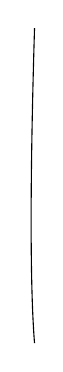
\begin{tikzpicture}\draw (0,0) .. controls (-.08,1) and (-.03,3) .. (0,4);\end{tikzpicture}}
De plus, pour les opérations tensorielles du type $\Lambda^i,\Gamma^i,\mathrm{Sym}^i$, elles manquent purement et simplement dans $\mathrm{Ab}_{h\cdot}$ (sauf de les définir par transport de structure via DP !) alors qu’elles sont \unsure{évidentes} \deleted{\unsure{pour}} sur $\mathrm{Ab}_{h*}$ ! Or ces structures également joueront un rôle essentiel par la suite.

\scanpage{320}
\[
\diagram{\begin{tikzcd}
\deleted{\unsure{F_A}(\Gamma^{pq}(X))}\arrow[r]&{}
\end{tikzcd}}
\]
\margin{$\Gamma^{pq}(f)\circ u_{pq}$}
\[
\diagram{\begin{tikzcd}[column sep=large,row sep=large]
\Gamma^{pq}(F_A(X))\arrow[r,"\sigma_{pq}^X"]\arrow[d]&F_A(\Gamma^{pq}(X))&{}\\
\Gamma^p(\Gamma^q(F_A(X)))\arrow[r,"\Gamma^p(\sigma_q^X)"]&\Gamma^p F_A\Gamma^q(X)\arrow[r]&F_A(\Gamma^p\Gamma^q(X))
\end{tikzcd}}
\]
\inserted{$\unsure{f^{pq}}$}
\margin{$f^{\unsure{(rs)|(pq)}}\in$}
\margin{$(f^{(q)})^{(p)}$}
\inserted{$(\Gamma^q(f)\circ u_q)^{(p)}$}
\deleted{$\unsure{F_A\Gamma^p(\Gamma^q(X))}$}
\margin{$F_A(\sigma_{p,q}^X)$}
\figure{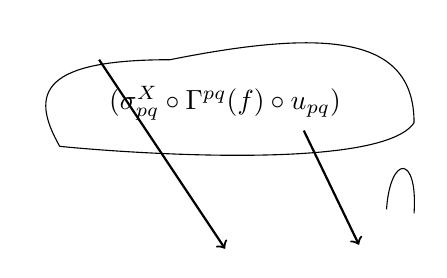
\begin{tikzpicture}
\node at (2.1,.55) {$(\sigma_{pq}^X\circ\Gamma^{pq}(f)\circ u_{pq})$};
\draw (0,0) .. controls (-.4,.7) and (-.2,1.1) .. (1.4,1.1) .. controls (3.4,1.5) and (4.5,1.4) .. (4.5,.3) .. controls (4.1,-.3) and (1,-.1) .. (0,0);
\draw[->,thick] (.5,1.1)--(2.1,-1.3);
\draw[->,thick] (3.1,.2)--(3.8,-1.25);
\draw (4.15,-.8) .. controls (4.2,-.1) and (4.55,-.1) .. (4.5,-.85);
\end{tikzpicture}}
\inserted{$\Gamma^p(\Gamma^q(f)\circ u_q)\circ u_p$}

\[
\diagram{\begin{tikzcd}[column sep=large,row sep=large]
\unsure{A'|A}\arrow[r,"u_{pq}"]\arrow[dd,"u_p"']&\Gamma^{pq}(A)\arrow[r,"\Gamma^{pq}(f)"]&\Gamma^{pq}(X)\arrow[d,"\sigma_{pq}^X"]\\
{}&{}&\Gamma^p(\Gamma^q(X))\\
\Gamma^p(A)\arrow[r,"\Gamma^p(u_q)"']\arrow[urr,bend left=12]&\Gamma^p(\Gamma^q(A))\arrow[ur]\arrow[r,draw=none,"\deleted{\longrightarrow}" description]&\deleted{\unsure{\Gamma^p(\Gamma}}\vphantom{\Gamma^q(A)}
\end{tikzcd}}
\]
\inserted{$\Gamma^p(\Gamma^q(f))$}
\deleted{$\unsure{\longrightarrow}$}
\margin{$f:A\longrightarrow X$}
\margin{$\Gamma^q f:\Gamma^q A\longrightarrow\Gamma^q X$}
\margin{$\Gamma^q f\circ u_q$}
\[
\diagram{\begin{tikzcd}
{}&\unsure{u_q}\\
A\arrow[ur,no head]&{}
\end{tikzcd}}
\]

$X=A,\ f=\mathrm{id}_A$
\[
\diagram{\begin{tikzcd}[column sep=large,row sep=large,execute at end picture={\draw (current bounding box.center) ellipse [x radius=3.8cm,y radius=2cm];}]
A\arrow[r,"u_{pq}"]\arrow[d,"u_p"']&\Gamma^{pq}(A)\arrow[d,"\sigma_{pq}^A"]\\
\Gamma^p(A)\arrow[r,"\Gamma^p(u_q)"']&\Gamma^p(\Gamma^q(A))
\end{tikzcd}}
\]
\figure{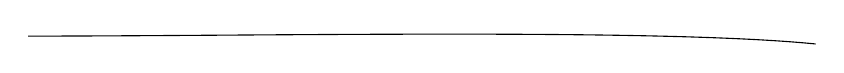
\begin{tikzpicture}\draw (0,0)..controls(3,0)and(8,.1)..(10,-.1);\end{tikzpicture}}

\[
\diagram{\begin{tikzcd}[column sep=large,row sep=large]
A\otimes A\arrow[r,"u_p\otimes u_q"]&\Gamma^p(A)\otimes\Gamma^q(A)\arrow[d,"\unsure{\beta_{p,q}^A}"]\\
A\arrow[u,"\Delta"]\arrow[r,"\unsure{c_{pq}|\gamma_{pq}}u_{p+q}"']&\Gamma^{p+q}(A)
\end{tikzcd}}
\]
\margin{$h\{T\}$}
\figure{\begin{tikzpicture}\draw[->] (.6,.7)--(0,0);\end{tikzpicture}}
\[
\boxed{u_p.u_q=\unsure{c_{pq}|\gamma_{pq}}u_{p+q}}\quad\text{dans }\operatorname{Hom}_{\unsure{1}}(A,\Gamma^*A)\simeq\unsure{(\operatorname{H}_{-},\mathrm{S}_\gamma\check A,\check A)}
\]
qui est une alg. grâce à la structure de coalg. sur $A$ et la structure d’alg. de $\Gamma^*A$
\[
\boxed{u_o=1}\qquad\boxed{u_1=\mathrm{id}}
\]
\figure{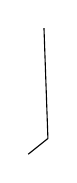
\begin{tikzpicture}\draw (0,.8)--(.05,-.6)--(-.2,-.8);\end{tikzpicture}}
\margin{321}

\scanpage{321}
\[
\diagram{\begin{tikzcd}
X\arrow[r,"\text{degré }n"]&Y\\
\Gamma^n(X)\arrow[ur]&{}
\end{tikzcd}}
\qquad F(X)\overset{?}{\unsure{-|\longrightarrow}}F(Y)
\]
\deleted{
\[
\diagram{\begin{tikzcd}
F(\Gamma^nX)\arrow[r,no head]&F(Y)\\
\Gamma^n(F(X))\arrow[u]\arrow[ur]&{}
\end{tikzcd}}
\]
\figure{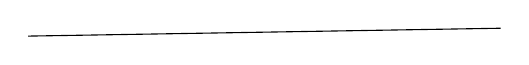
\begin{tikzpicture}\draw(0,0)--(6,.1);\end{tikzpicture}}
\[
F_A(X)=\operatorname{Hom}_A(X)
\]
\[
\diagram{\begin{tikzcd}
\Gamma^nF_A(X)\arrow[r,"?"]&F_A(\Gamma^nX)
\end{tikzcd}}
\]
\[
\diagram{\begin{tikzcd}
\Gamma^n\operatorname{Hom}_1(A,X)\arrow[r,"\unsure{\beta}?"]&\operatorname{Hom}_1(A,\Gamma^nX)
\end{tikzcd}}
\]
\deleted{$\unsure{\beta(u^{(n)})}\longrightarrow\unsure{A}\cdot\Gamma^n(f)$}
\unsure{foncteur} en $\unsure{A|X}$
\[
\unsure{Y|X}\longrightarrow X\otimes X
\]
\margin{bilin, \unsure{fonct.} en $X,Y$}
\[
\diagram{\begin{tikzcd}
F_{\unsure{C|A}}(X\otimes Y)&F_A(X)\times F_{\unsure{B|A}}(Y)\arrow[l]
\end{tikzcd}}
\]
\inserted{$\unsure{\varphi}$}
: si $X=Y=A$, l’image $\mathrm{id}_A,\mathrm{id}_A$ donne un élt
\[
A\longrightarrow A\otimes A
\]
\unsure{comparer}

a) associativité : \unsure{associativité} de la coalg.

b) \uline{commutativité}

c) compatible avec $1$ i.e.
\[
\diagram{\begin{tikzcd}
\unsure{k_\varphi|h_\varphi}\arrow[r]&F_A(1)=\\
{}&\operatorname{Hom}(A,1)\arrow[u,equals]
\end{tikzcd}}
\]
\unsure{re.}\quad\unsure{coaugm}\quad $A\overset{u}{\longrightarrow}1$
\figure{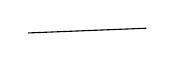
\begin{tikzpicture}\draw (0,0)--(1.5,.06);\end{tikzpicture}}
}
\figure{\begin{tikzpicture}\draw(0,8)--(4,0);\end{tikzpicture}}
\margin{322}

\scanpage{322}
\deleted{$\Gamma^p(f)\circ u_p$}
\deleted{$\Gamma^p(f)$}
\[
\diagram{\begin{tikzcd}[column sep=large,row sep=large]
\Gamma^p(F_A(X))\otimes\Gamma^q(F_A(\unsure{X|Y})))\arrow[r]\arrow[d]&F_A\Gamma^p(X)\otimes F_A\Gamma^q(\unsure{X|Y})\arrow[d]\\
\Gamma^{p+q}F_A(X)\arrow[r,no head]\arrow[d]&\unsure{F_A\Gamma^{p+q}F(X)}\\
[(\Gamma^p f\circ u_p)\otimes(\Gamma^q g\circ u_q)]\circ\Delta&{}
\end{tikzcd}}
\]
\[
f,g:\diagram{\begin{tikzcd}A\arrow[r,shift left=.5ex]\arrow[r,shift right=.5ex,"{1,1}"']&X\end{tikzcd}}
\]
\[
(\Gamma^p f\circ u_p\quad\unsure{\otimes}\quad\Gamma^q g\circ u_q)
\]
\[
A\longrightarrow\Gamma^p X\qquad A\longrightarrow\Gamma^q X
\]
\[
f^{(p)}\otimes g^{(p)}
\]
\[
\diagram{\begin{tikzcd}[column sep=large,row sep=huge]
A\arrow[r,"\Delta"]\arrow[d]\arrow[drr,bend right=15,"{\text{défini par }f^{(p)}g^{(q)}\in\Gamma^{p+q}F_A(X)}"']&A\unsure{\otimes}A\arrow[r,"{(\Gamma^p f\circ u_p^{\unsure{A}})\otimes(\Gamma^qg\circ u_q)}"]&\Gamma^p(X)\otimes\Gamma^q(Y)\arrow[d]\\
{}&{}&\Gamma^{p+q}(X)
\end{tikzcd}}
\]
\margin{$f^{(p)}\otimes g^{(q)}$}
\[
\diagram{\begin{tikzcd}[column sep=huge,row sep=large]
\Gamma^p(\overbrace{F_A(X)}^{f})\otimes\Gamma^q(\overbrace{F_A(X)}^{g})\arrow[r]\arrow[d]&F_A\Gamma^p(X)\otimes F_A\Gamma^q(X)\\
\Gamma^{p+q}F_A(X)\arrow[ddr]&F_A(\Gamma^p(X)\otimes\Gamma^q(X))\arrow[u,"\unsure{\uparrow|\downarrow}"]\arrow[d]\\
{}&F_A(\Gamma^{p+q}(X))\\
{}&{}
\end{tikzcd}}
\]
\margin{$f^{(p)}\in$}
\margin{$\ni g^{(q)}$}
\margin{$\Gamma^p(f)\circ u_p\quad\otimes\quad\Gamma^q(g)\circ u_q$}
\margin{$f^{(p)}g^{(q)}$}
\inserted{$\unsure{\wedge}$}

Il suffit de prendre $X=Y=A$, $f=g=\mathrm{id}$
\[
\diagram{\begin{tikzcd}[column sep=large,row sep=huge]
A\arrow[r,"\Delta"]\arrow[drr,bend right=15,"{\text{défini par }(\mathrm{id}_A)^{(p)}(\mathrm{id}_A)^{(q)}\in\Gamma^{p+q}F_A(A)}"']&A\otimes A\arrow[r,"u_p\otimes u_q"]&\Gamma^p(A)\otimes\Gamma^q(A)\arrow[d]\\
{}&{}&\Gamma^{p+q}(A)
\end{tikzcd}}
\]
\margin{$1^{(p)}1^{(q)}=c_{pq}1^{(p+q)}$}
i.e. par $c_{pq}\mathrm{id}_A^{(p+q)}$, donc $\unsure{c_{p+q}|c_{pq}}u_{p+q}$
\figure{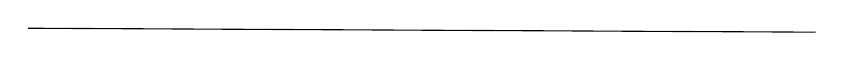
\begin{tikzpicture}\draw(0,0)--(10,-.05);\end{tikzpicture}}
\[
\diagram{\begin{tikzcd}[column sep=large]
\underbrace{\Gamma^*F(\unsure{A})}_{\otimes\text{-anneau}}\arrow[r]&\underbrace{F(\unsure{F^*|\Gamma^*}(X))}_{\otimes\text{-anneau}}
\end{tikzcd}}
\]
car $F$ commute à $\otimes$
\figure{\begin{tikzpicture}\draw(0,0)--(0,1);\end{tikzpicture}}
\margin{323}

\scanpage{323}
$(\unsure{1})\Longleftrightarrow(\unsure{3})$ déjà vu.

$(2)\Longleftrightarrow(\unsure{3})$ La donnée d’un hom de foncteurs cov
\[
F_A\overset{u}{\longrightarrow}\deleted{\unsure{\mathrm{End}}}\ G=F_A\circ\Gamma^p
\]
équivaut à la donnée d’un élt
\[
u_p\in\unsure{G_A|G}(A)=\operatorname{Hom}(A,\Gamma^p(A))
\]
Il faut exprimer les cond. de (2).
\inserted{Les \unsure{égalités} $f^{(0)}=1$, $f^{(1)}=0$ expriment $\unsure{u_0}=1$, $\unsure{u_1}=\mathrm{id}$.}
La relation $(f+g)^{(p)}=\sum f^{(i)}g^{(j)}$ : il suffit de voir le cas universel
\[
M=A\times A,\quad f=\mathrm{inj}_1=\alpha,\quad g=\mathrm{inj}_2=\beta,
\]
\[
\unsure{(f+g)^\beta|(f+g)}=\Delta:A\longrightarrow A\times A=M
\]
\[
(f+g)^{\unsure{n|p}}=\Gamma^p(\Delta)\circ u_p\quad\deleted{\unsure{\Gamma^p(A)}}\longrightarrow\Gamma^p(M)
\]
\[
\diagram{\begin{tikzcd}[column sep=large,row sep=large]
A\arrow[r,"u_p"]\arrow[d,"\Delta_A^{\unsure{(p)}}"']&\Gamma^p(A)\arrow[r,"\Gamma^p(\Delta_A)"]\arrow[dr,"\Delta_{\Gamma^*A}"]&\Gamma^p(A\unsure{\oplus|\times}A)\arrow[d,"\simeq"]\\
\underbrace{A\times-\times A}_{p}\arrow[rr]&{}&\displaystyle\sum_{i+j=p}\Gamma^{\deleted{\unsure{p}}i}A\otimes\Gamma^jA
\end{tikzcd}}
\]
\margin{\unsure{car} $A\longrightarrow\Gamma^i(A)\otimes\Gamma^j(A)$}
\figure{\begin{tikzpicture}\draw (0,.8)..controls(-.3,.6)and(-.2,.3)..(0,0);\draw(2,.8)..controls(2.3,.4)and(2.3,0)..(2,-.2);\end{tikzpicture}}
On trouve $\Delta(u_p)=\displaystyle\sum_{i+j=p}\unsure{u^i|u_i}\otimes u_j$
\margin{324}

\scanpage{324}
Deux questions de p.d. (la \unsure{première} connue)

\textcircled{1} Soit $A$ une coalgèbre \unsure{ass counit comm} $(B,J)$, une algèbre à p.d. : p.e. (p.ex $(\Gamma^*M,\Gamma^+M)$) de sorte que $\operatorname{Hom}_h(A,M)$ a une structure d’anneau --- ou de $h$-algèbre, et $\operatorname{Hom}_h(A,J)$ en est un idéal. (Si $A$ est libre de type fini, on trouve l’anneau $\check A\otimes B$ avec l’idéal $\check A\otimes J$,) qui a des p.d.) Cet idéal a-t-il des p.d. ?

\deleted{\textcircled{\unsure{2}}} Prenons $B=\Gamma^*A$, $J=\Gamma^+A$, et soit $u_1\in\operatorname{Hom}_h(A,B)$ l’application identique $A\longrightarrow A$. Considérons les $u_n=u_1^{(n)}$. satisfont-ils
\[
\sigma_{pq}^A\circ u_{pq}=\Gamma^p(u_q)\circ u_p\quad ?
\]
Sont ils (pour $u_1$ fixé) les seuls éléments \unsure{hom} satisfaisant cette relation, plus $u_pu_q=c_{pq}u_{p+q}$, et pour lequel $u_1$ est comme dessus ?

\textcircled{2} Soit $A$ une \uline{algèbre}, \unsure{pour le cas commut}) $B$ une coalgèbre à copuissances divisées pour le \unsure{coker} de $B'\longrightarrow B$. (hom de coalgèbres) p.ex. $B=\mathrm{Sym}^*M$, prenant $\mathrm{Sym}^*(0)=h$ \unsure{---}. Donc sur $\operatorname{Hom}_h(B,A)$ il y a une structure de \deleted{p.d. \unsure{relti}} algèbre, à p. div. sur
\[
\operatorname{Ker}\ \operatorname{Hom}_{\unsure{h|k}}(B,A)\unsure{\mathrel{-}|\longrightarrow}\operatorname{Hom}_{\unsure{h|k}}(B',A).
\]
\margin{325}

\scanpage{325}
3) Donnée d'une application (pour tt $p\geq0$)
\[
\operatorname{Hom}_h(A,M)\xrightarrow{\unsure{u_A^{(p)}|u_A^p}}\operatorname{Hom}_h(A,\Gamma^p M)
\]
(pas \inserted{néc.} lin) fonctorielle en $M$, notée
ce qui \deleted{fait} sera noté
\[
f\longmapsto f^{(p)}
\]
et satisfaisant les relations $f^{(0)}=1$, $f^{(1)}=f$, et
\[
\left\{\begin{aligned}
(f+g)^{(p)}&=\sum_{\unsure{i+j=0|i+j=p}} f^{(i)}g^{(j)}\\
(\lambda f)^{(p)}&=\lambda^p f^p\quad\text{(automatique!)}
\end{aligned}\right.
\]
et ---

4) Donnée d'une loi de p.d. sur
\[
\operatorname{Hom}_h(A,\Gamma^+M)\subset\operatorname{Hom}_h(A,M)
\]
$\forall M$, fonctorielle en $M$, et telle que

5) Loi à p.d. sur $\operatorname{Hom}(A,\Gamma^+A)\subset\operatorname{Hom}(A,\Gamma^*A)$
\margin{(\unsure{en. commut|an. commut})}

6) Donnée, pour tte $h$-algèbre $B$ (avec
idéal $J$ à p.d, d'une loi de
p.d. sur $\operatorname{Hom}_h(A,J)\subset\operatorname{Hom}_h(A,B)$,
fonctorielle en $(B,J)$ $\ldots\ldots$
\figure{\begin{tikzpicture}\draw (0,0)--(0,1.7);\draw (.3,.1)--(.3,1.65);\end{tikzpicture}}
\margin{326}

\scanpage{326}
\deleted{\diagram{\begin{tikzcd}
\unsure{\mathrm{G\ell}(2,\mathbb C)}\arrow[r]\arrow[d]&\unsure{\mathrm{GP}(1,\mathbb C)}\arrow[d]\\
\unsure{\mathbb C^*}&\unsure{\mathbb C^*}\\
\unsure{\mathrm{SL}(2,\mathbb C)}\arrow[uur]&
\end{tikzcd}}}
\[
\unsure{c_2^*}\qquad\tfrac12\unsure{c_2^*}=c'_2
\]
\diagram{\begin{tikzcd}[column sep=small,row sep=small]
1\arrow[r]&\mu_2\arrow[r]&\mathrm{SL}(2,\mathbb C)\arrow[rr]\arrow[dd]&{}&\mathrm{GP}(1,\mathbb C)\arrow[dd]\arrow[r,dash]&1\\
{}&{}&{}&\begin{gathered}\mathrm T_{\mathbb C}\quad c_1\\\unsure{\mathrm{SO}(2,\mathbb C)}\simeq\mathrm G_m\end{gathered}\arrow[ul]\arrow[dd,leftrightarrow]&{}&{}\\
1\arrow[r,dash]&\mu_2\arrow[uu]\arrow[r]&\mathrm{SL}(2,\mathbb R)\arrow[rr]&{}&\mathrm{GP}(1,\mathbb R)\arrow[r,dash]&1\\
{}&{}&E_1&\begin{gathered}\mathrm T_{\mathbb R}^{o}\simeq\underset{c_1}{\mathbb S^1}\\\Vert\\\mathrm{SO}(2,\mathbb R)\end{gathered}\arrow[ul]&\tfrac12 E_1=E'_1&{}
\end{tikzcd}}
\[
\boxed{\begin{pmatrix}a&b\\-b&a\end{pmatrix}\quad a^2+b^2=1}
\]
\[
\underbrace{(a+ib)}_{\deleted{\unsure{b+ia}}\;\lambda}
\underbrace{(a-ib)}_{\mu}=1\qquad\lambda\mu=1
\]
\[
a=\frac{\lambda+\mu}{2}=\deleted{\unsure{\frac{\lambda+\lambda}{2}}}\frac12(\lambda+\lambda^{-1})
\qquad
b=\frac{\lambda-\mu}{2i}=\frac12(\lambda-\lambda^{-1})
\]
\[
\Omega\otimes\Omega\qquad\deleted{a+i}
\]
\[
\Omega\qquad\underbrace{\mathrm P\bigl(\underbrace{\Omega+\Omega^{-1}}_{}\bigr)}_{}
\]
\[
\underbrace{\Omega^{-1}\quad\Omega^{-2}}_{}\big/\underbrace{\Omega,\quad\unsure{\mathcal O|0}}_{}
\]
\[
\mathrm P^3\qquad\underbrace{\Omega^2\quad\Omega}_{}\quad\uline{\unsure{\mathcal O|0}}
\qquad\underbrace{\Omega\quad\uline{\unsure{\mathcal O|0}}}_{}
\]
\[
\unsure{H^1(X,\Omega)\simeq\mathbb C|H^1(X,\mathbb R)\simeq\mathbb C}
\]
\margin{$\Omega_{\unsure{C|S}}^{n-1}$}
\diagram{\begin{tikzcd}
{}\arrow[r,dash]&\Omega^n\arrow[r]&\mathrm P_{X/h}^n\arrow[r,dash]&\mathrm P_{X/h}^{n-1}\arrow[r]&0
\end{tikzcd}}
\[
\Omega\qquad\uline{\unsure{\mathcal O|0}}
\]
\figure{\begin{tikzpicture}
\draw (0,0)--(3.3,1.8) .. controls (3.7,2.1) and (3.6,2.7) .. (3.7,3.5) -- (3.7,5.2) .. controls (3.6,5.7) and (4,5.8) .. (5.2,6.1);
\end{tikzpicture}}
\diagram{\begin{tikzcd}
\mathrm{G\ell}\arrow[r]&\uline{\mathrm{G.P}}\\
\mathrm P\arrow[r]\arrow[d,dash]&\mathrm P'\arrow[d,dash]\\
\check E&\mathcal O_X\arrow[l]
\end{tikzcd}}
\[
\textcircled{\unsure{n}}
\]
\diagram{\begin{tikzcd}
E\arrow[r,"\text{épi}"]&\mathcal O_X
\end{tikzcd}}
\[
\unsure{a_n f^{(n)}+a_{n-1}f^{(n-1)}}\quad-\unsure{a_1 f^{(1)}}-a_0f=0
\]
\diagram{\begin{tikzcd}
E\arrow[r]\arrow[d,bend right=15]&E\otimes\Omega^1_{X/S}\\
\mathrm P^n_{X/h}\arrow[r,"D"]&\unsure{\mathcal O_X}
\end{tikzcd}}
\[
E\mathrel{-}\mathcal O_X\qquad Df+\uline{\alpha}f=0
\]
\[
\mathrm P^n_{X/h}\unsure{\simeq|=}\mathcal O_X+\mathrm P^{n+}_{X/h}
\]
\[
\underbrace{\mathrm{Sym}^n\Omega^1}_{}
\]
\figure{\begin{tikzpicture}
\draw (0,1.4) .. controls (0.15,1.4) and (0.15,0.8) .. (0,0.8) .. controls (-0.2,0.8) and (-0.2,0.7) .. (0,0.7) .. controls (0.15,0.7) and (0.15,0) .. (0.4,0);
\draw (0.4,0)--(0.05,0.03);
\draw (0.5,0.45)--(2.7,0.45);
\end{tikzpicture}}
\margin{327}

\scanpage{327}
$X$ courbe alg. $/\mathbb C$ \unsure{propre non sing connexe}, genre $g\geq2$.
Il y a sur $X$ un \deleted{fibré principal}\inserted{torseur} canonique
$P$ de \unsure{gr.} $\mathrm{GP}(1)_{\mathbb C}=G'_{\mathbb C}$ à connexion intégrable
(compatible à structure de torseur), obtenu ainsi:
$\forall x\in X\longmapsto\widetilde X(x)$ rev. universel de $X$ en $x$
\[
\widetilde X(x)\unsure{\longleftrightarrow|\simeq}
\deleted{\unsure{demi-plan disque}}\inserted{demi-plan de}\text{ Poincaré }D
\]
ens. des iso $\operatorname{Iso}\bigl((D,0),\widetilde X(x,\widetilde x)\bigr)$ est un torseur à droite
sur $\unsure{\widehat{\operatorname{Isot}}|\operatorname{Isot}}(D,0)\simeq
\deleted{\mathrm{GP}(1)_{\mathbb R}\simeq G'_{\mathbb C}}\inserted{S_{\mathbb R}}$,
d'où par \unsure{ext.} un torseur à droite sur $G'$, \inserted{soit $P_x$.}
\deleted{\unsure{ceci dit par $G_0$}}.
\margin{\unsure{On}}

On \unsure{sait|voit} que les $P_x$ ($x\in X(\mathbb C)$) sont les fibres
d'un fibré principal \deleted{analytique}\inserted{top.} à structure \unsure{plat|plate}
(celui associé à $\pi_{\unsure{x|1}}\longrightarrow G'_{\mathbb R}\subset G'_{\mathbb C}$)

\uline{Th} $\forall x\in X$, $\exists$ une et une seule \deleted{\unsure{imm.}}\inserted{\unsure{imm.}}
\unsure{ouverte} analytique de $\widetilde X(x)$ dans
$T_x(X)$ dont a) l'image est un disque
b) l'application tangente en $\widetilde x$ est l'identité.
\figure{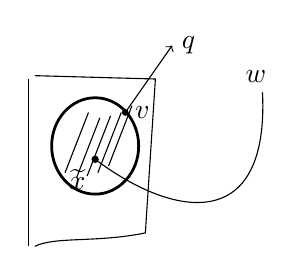
\begin{tikzpicture}[scale=.85]
\draw (0,0)--(0,2.5);\draw (.1,2.55)--(1.9,2.5)--(1.75,.2).. controls (1,.05) and (.4,.15) .. (.1,0);
\draw[line width=1pt] (1,1.5) ellipse (.65 and .72);
\foreach \x/\y in {.55/1.1,.72/1.02,.88/1.05,1.04/1.1,1.2/1.2}{\draw (\x,\y)--(\x+.35,\y+.9);}
\fill (1,1.3) circle (.055);\node[below left] at (1,1.3) {$\widetilde x$};
\fill (1.45,2) circle (.05);\node[right] at (1.45,2) {$\unsure{v}$};
\draw[->] (1.45,2)--(2.15,3);\node[right] at (2.15,3) {$\unsure{q}$};
\draw (1,1.3) .. controls (2.2,.4) and (3.6,.2) .. (3.5,2.3);\node[above] at (3.4,2.3) {$\unsure{w}$};
\end{tikzpicture}}
\[
\pi_1(X,x)\subset G'\subset G'_{\mathbb C}
\]
\figure{\begin{tikzpicture}\draw[->] (0,.6)--(.1,0);\node[below] at (.1,0) {$\unsure{u}$};\end{tikzpicture}}
\[
\begin{pmatrix}a&b\\c&d\end{pmatrix}\mathbin{.}z=
\qquad
\begin{array}{cc}a^{\unsure{*}}&b\\-b&a\end{array}
\]
\[
\deleted{\unsure{\mathrm{Iso}}}\uline{P(x,q)}
\]
\[
P(x,\varphi q)=P(x,q)\mathop{\wedge}_{i_{\varphi}}G'_{\mathbb C}
\]
\[
\unsure{\varphi\in S'_{\mathbb C}\subset G'\subset G'_{\mathbb C}}
\qquad\mathbb C^*
\]
\diagram{\begin{tikzcd}
P(x,q)\arrow[d,"\unsure{z}"']&G'_{\mathbb C}\arrow[d,"\unsure{i_{\varphi}}"]\\
P(x,\unsure{x'|u'})&G'_{\mathbb C}
\end{tikzcd}}
\diagram{\begin{array}{ccc}
Q_{\mathbb R}& &\textcircled{$P_{\mathbb R}$}\\
&S_{\mathbb R}\subset&G'_{\mathbb R}\\
&\cap&\cap\\
Q_{\mathbb C}&S_{\mathbb C}\subset&G'_{\mathbb C}\quad P_{\mathbb C}
\end{array}}
\figure{\begin{tikzpicture}
\draw (.4,2.5).. controls (-.2,2) and (-.2,1.4) .. (.3,1);
\draw (0,.3)--(0,0)--(3,0)--(3.05,.3);
\end{tikzpicture}}
\margin{$P(x,\varphi\unsure{q})=P(x,\unsure{x|u})\mathop{\wedge}_{i_{\varphi}}G'_{\mathbb C}$}
\diagram{\begin{tikzcd}
\mathbb C^*\subset\mathrm{G\ell}(2,\mathbb R)\arrow[d]\\
\mathrm{G\ell}(2,\mathbb C)
\end{tikzcd}}
\margin{$G_m\longrightarrow\unsure{\mathrm{GP}_{\mathbb R}|\mathrm{GP}_2}$}
\diagram{\begin{tikzcd}E\arrow[r]&E\otimes\Omega\end{tikzcd}}
\figure{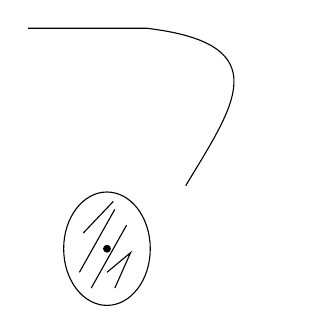
\begin{tikzpicture}
\draw (0,2)--(1.5,2) .. controls (3.2,1.8) and (2.6,1) .. (2,0);
\draw (1,-.8) ellipse (.55 and .72);
\fill (1,-.8) circle (.05);
\draw (.65,-1.1)--(1.1,-.3);\draw (.8,-1.3)--(1.25,-.5);\draw (.7,-.6)--(1.08,-.2);\draw (1,-1.1)--(1.3,-.85)--(1.1,-1.3);
\end{tikzpicture}}
\diagram{\begin{tikzcd}E\arrow[r]&E\otimes\Omega\end{tikzcd}}

 a) fibré inversible: $\uline{\Omega^{-1}}$

 b) \deleted{\unsure{fibré}} $\mathrm P(\Omega^{-1}+\Omega)$ avec conn. intégrable
\[
\begin{pmatrix}\Omega&0\\\Omega^3&\Omega\end{pmatrix}
\]
\figure{\begin{tikzpicture}\draw (0,2)--(2,2).. controls (2.7,2) and (2.4,.8) .. (3,0);\end{tikzpicture}}
\[
\boxed{\begin{gathered}
\text{Trouver une connexion intégrable}\\
\text{(alg) canonique sur}\\
\mathrm P(\Omega^{-1}+\Omega)=\overline{\mathrm V(\Omega^2)}
\end{gathered}}
\]
\[
\Omega^{-1}\oplus\Omega\longrightarrow(\Omega^{-1}\oplus\Omega)\otimes\Omega
=\unsure{\Omega_X^0|\mathcal O_X}+\Omega^2
\]
\[
\unsure{(D,\omega)=(d,\overline\omega,\Delta)}
\]
\figure{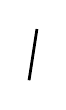
\begin{tikzpicture}\draw[line width=1pt] (0,0)--(.1,.65);\end{tikzpicture}}
\margin{328}
